%# -*- coding: utf-8-unix -*-
%%==================================================

\chapter{预备知识}

在了解疲劳检测相关研究之前,我们先要了解下面三个容易混淆的术语:数据分析,机器学习和数据科学。因为不管是在学术界,还是在企业界,这三个术语始终贯穿在近代科学技术发展的过程中,在疲劳检测的发展过程也是如此。因此如果我们对这些术语能够有所区分,有所理解,一方面能够帮助我们在疲劳检测研究中理清研究思路,优化研究步骤,另一方面能够帮助我们更清楚地定位自己,为自己以后找怎样的工作做准备。

\section{数据分析}

\subsection{数据分析的定义}

数据分析是指用适当的统计分析方法对收集来的大量数据进行分析,将它们加以汇总和理解并消化,以求最大化地开发数据的功能,发挥数据的作用。数据分析是为了提取有用信息和形成结论而对数据加以详细研究和概括总结的过程。这里的数据也称观测值,是通过实验、测量、观察、调查等方式获取的结果,常常以数量的形式展现出来。

数据分析的目的是把隐藏在一大批看似杂乱无章的数据背后的信息集中和提炼出来,总结出所研究对象的内在规律。在实际工作中,数据分析能够帮助管理者进行判断和决策,以便采取适当策略与行动。例如,企业的高层希望通过市场分析和研究,把握当前产品的市场动向,从而制订合理的产品研发和销售计划,这就必须依赖数据分析才能完成。

在统计学领域,有些学者将数据分析划分为描述性数据分析、探索性数据分析以及验证性数据分析。其中,探索性数据分析侧重于在数据之中发现新的特征,而验证性数据分析则侧重于验证已有假设的真伪证明。

从另一个角度看,描述性数据分析属于初级数据分析,常见的分析方法有对比分析法、平均分析法、交叉分析法等。而探索性数据分析以及验证性数据分析属于高级数据分析,常见的分析方法有相关分析、因子分析、回归分析等。

\subsubsection{数据分析和数据处理的区别}

数据处理是数据分析的基础。通过数据处理,将收集到的原始数据转换为可以分析的形式,并且保证数据的一致性和有效性。如果数据本身存在错误,那么即使采用最先进的数据分析方法,得到的结果也是错误的,不具备任何参考价值,甚至还会误导决策。

\subsubsection{数据分析和数据挖掘的区别}

数据分析可以分为广义的数据分析和狭义的数据分析。在广义的数据分析中,数据分析包括狭义的数据分析和数据挖掘,数据挖掘是一种高级的数据分析方法。我们常说的数据分析是指狭义的数据分析,它和数据挖掘还是有些区别的\footnote{\url{https://www.zhihu.com/question/20127962/answer/130339113}}。

数据挖掘就是从大量的数据中挖掘出有用的信息,它是根据用户的特定要求,从浩如烟海的数据中找出所需的信息,以满足用户的特定需求。数据挖掘技术是人们长期对数据库技术进行研究和开发的结果。一般来说,数据挖掘侧重解决四类数据分析问题:分类、聚类、关联和预测,重点在寻找模式与规律。

它们之间的主要区别是\footnote{\url{https://www.zhihu.com/question/20127962/answer/23794384}}:
\begin{enumerate}
	\item "数据分析"的重点是观察数据,而"数据挖掘"的重点是从数据中发现"知识规则"KDD(Knowledge Discover in Database)。
    \item "数据分析"得出的结论是人的智力活动结果,而"数据挖掘"得出的结论是机器从学习集(或训练集、样本集)发现的知识规则。
    \item "数据分析"得出结论的运用是人的智力活动,而"数据挖掘"发现的知识规则,可以直接应用到预测。
    \item "数据分析"不能建立数学模型,需要人工建模,而"数据挖掘"直接完成了数学建模。如传统的控制论建模的本质就是描述输入变量与输出变量之间的函数关系,“数据挖掘”可以通过机器学习自动建立输入与输出的函数关系,根据KDD得出的“规则”,给定一组输入参数,就可以得出一组输出量。
\end{enumerate}

数据分析一般都是得到一个指标统计量结果,如总和、平均值等,这些指标数据都需要与业务结合进行解读,才能发挥出数据的价值与作用。而数据挖掘输出结果是模型或规则,并且可相应得到模型得分或标签,模型得分如流失概率值、总和得分、相似度、预测值等,标签如高中低价值用户、流失与非流失、信用优良中差等。

举个简单的例子:有一些人总是不及时向电信运营商缴钱,如何发现它们?

\begin{itemize}
    \item 数据分析:通过对数据的观察,我们发现不及时缴钱人群里的贫困人口占82$\%$。所以结论是收入低的人往往会缴费不及时。结论就需要降低资费。
    \item 数据挖掘:通过编写好的算法自行发现深层次的原因。原因可能是,家住在五环以外的人,由于环境偏远不及时缴钱。结论就需要多设立一些营业厅或者自助缴费点。
\end{itemize}

狭义数据分析与数据挖掘的本质是一样的,都是从数据里面发现关于业务的知识,从而帮助业务运营、改进产品以及帮助企业做更好的决策。

\subsection{数据分析的作用}

这里主要介绍数据分析在企业的日常经营分析中的三大作用。

1、现状分析: 简单来说就是告诉你过去发生了什么。

第一,告诉你企业现阶段的整体运营情况,通过各个经营指标的完成情况来衡量企业的运营状态,以说明企业整体运营是好了还是坏了,好的程度如何,坏的程度又到哪里。

第二,告诉你企业各项业务的构成,让你了解企业各项业务的发展及变动情况,对企业运营状况有更深入的了解。

现状分析一般通过日常通报来完成,如日报、周报、月报等形式。\\

2、原因分析:简单来说就是告诉你某一现状为什么发生。

经过第一阶段的现状分析,我们对企业的运营情况有了基本了解,但不知道运营情况具体好在哪里,差在哪里,是什么原因引起的。这时就需要开展原因分析,以进一步确定业务变动的具体原因。例如2020 年2月运营收入环比下降5$\%$,是什么原因导致的呢?是各项业务收入都出现下降,还是个别业务收入下降引起的?是各个地区业务收入都出现下降,还是个别地区业务收入下降引起的?这就需要我们开展原因分析,进一步确定收入下降的具体原因,对运营策略做出调整与优化。

原因分析一般通过专题分析来完成,根据企业运营情况选择针对某一现状进行原因分析。\\

3、预测分析:简单来说就是告诉你将来会发生什么。

在了解企业运营现状后,有时还需要对企业未来发展趋势作出预测,为制订企业运营目标及策略提供有效的参考与决策依据,以保证企业的可持续健康发展。

预测分析一般通过专题分析来完成,通常在制订企业季度、年度等计划时进行,其开展的频率没有现状分析及原因分析高。

\subsection{数据分析方法论}

数据分析方法论主要用来指导数据分析师进行一次完整的数据分析,它更多的是指数据分析思路,比如主要从哪几方面开展数据分析?各方面包含什么内容和指标?
所以,数据分析方法论主要从宏观角度指导如何进行数据分析,它就像是一个数据分析的前期规划,指导着后期数据分析工作的开展。而数据分析法则是指具体的分析方法,例如我们常见的对比分析、交叉分析、相关分析、回归分析、聚类分析等数据分析法。数据分析法主要从微观角度指导如何进行数据分析。

很多人在做数据分析时,经常遇到这几个问题:不知从哪方面入手开展分析;分析内容和指标常常被质疑是否合理、完整,而自己也说不出个所以然来。对这些问题常常感到困扰。这就是为什么强调数据分析方法论的原因,刚才也说过数据分析方法论主要用来指导数据分析师进行一次完整的数据分析,而只有在营销、管理等方法和理论的指导下,结合实际业务情况,才能确保数据分析维度的完整性,分析结果的有效性及正确性。

数据分析方法论主要有以下几个作用。
\begin{itemize}
	\item 理顺分析思路,确保数据分析结构体系化。
    \item 把问题分解成相关联的部分,并显示它们之间的关系。
    \item 为后续数据分析的开展指引方向。
    \item 确保分析结果的有效性及正确性
\end{itemize}

企业界中有几种常见的数据分析方法论:PEST分析法,5W2H分析法,逻辑树分析法,4P营销理论和用户行为理论,这些方法论可以帮助我们按照某种分析思路,较为全面地找准分析对象,并建立不同分析对象间的内在关系,目的是为了让我们最终的分析报告在整体上更有逻辑性,更能以理服人。这些方法论的最终目的是为了找到公司在某方面存在的不足,并且通过数据分析师的合理决策让公司去弥补这些不足(比如营业额增长缓慢,用户流失严重等)。

业界的这些方法论并不完全适用于学术界,但对于创新性的实验分析过程的展开具有一定的启发和指导意义。以驾驶员疲劳检测为例,要想开展这方面的实验研究,我们首先要了解驾驶员疲劳检测的发展现状,就好比数据分析师在进行数据分析之前,要先了解公司内部业务一样。接着我们要能够通过阅读其他人的论文,列举出该领域暴露的难点或问题,并以此作为突破口开展实验分析,就好比数据分析师通过对公司的现状分析发现公司存在的问题,并对该问题进行原因分析。数据分析师在进行原因分析之前,可以使用接下来要介绍的分析方法论,尽可能列举出所有要分析的对象(广告成本,用户阶层,网站平均访问量等)建立分析层次,这一点我们也可以效仿,比如我们可以通过分析眨眼频率,闭眼时间,心率,张嘴程度这些指标来估计疲劳。但是在相同环境下,眨眼频率,心率等特征也会因人而异,所以要对这些特征进行融合分析需要一定的分析层次和权重设置。

接下来我将对这些数据分析方法论进行一一介绍。

\subsubsection{PEST分析法}

PEST分析法用于对宏观环境的分析。宏观环境又称一般环境,是指影响一切行业和企业的各种宏观力量。对宏观环境因素作分析时,由于不同行业和企业有其自身特点和经营需要,分析的具体内容会有差异,但一般都应对政治(Political)、经济(Economic)、技术(Technological)和社会(Social)这四大类影响企业的主要外部环境因素进行分析,这种方法简称为PEST分析法。用PEST分析法对互联网行业进行分析示例如图\href{fig:1-1}{1-1}所示。

\begin{figure}[!htp]

\centering
%\begin{minipage}[t]{5in}
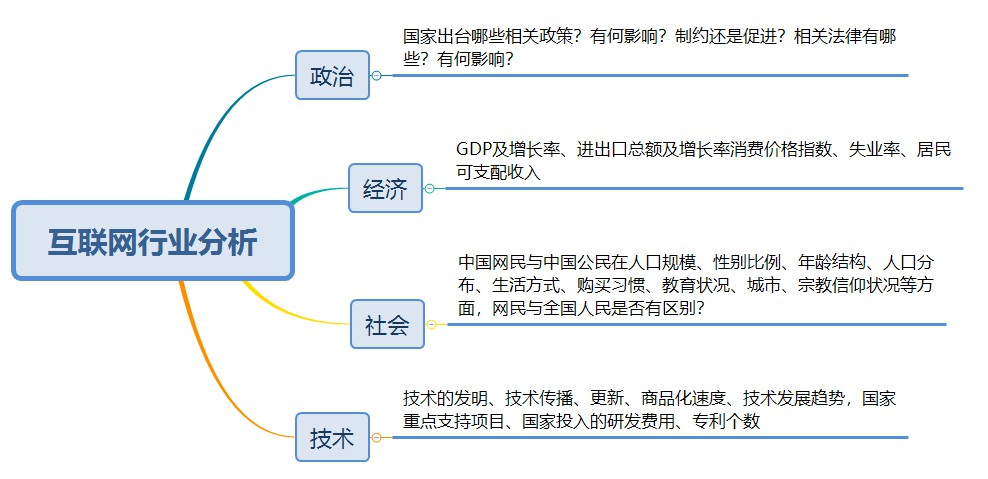
\includegraphics[width=5in]{example/PEST.JPG}
\caption{用PEST分析法对互联网行业进行分析示例}
\label{fig:1-1}
%\end{minipage}

\end{figure}

\subsubsection{5W2H分析法}

5W2H分析法是以五个W开头的英语单词和两个H开头的英语单词进行提问,从回答中发现解决问题的线索,即何因(Why)、何事(What)、何人(Who)、何时(When)、何地(Where)、如何做(How)、何价(How much),这就构成了5W2H分析法的总框架。

该方法简单、方便,易于理解和使用,富有启发意义,广泛用于企业营销、管理活动,对于决策和执行性的活动措施非常有帮助,也有助于弥补考虑问题的疏漏。其实对任何事情都可以从这七大方面去思考,对于不善分析问题的人,只要多练习即可上手,所以同样它也适用于指导建立数据分析框架。

现在以用户购买行为分析为例,来学习5W2H分析法。例如我们需要了解公司产品的用户购买行为是怎样的。这时可在5W2H分析法的指导下整理分析用户购买行为的思路,建立用户购买行为分析框架。如图\href{fig:1-2}{1-2}所示,根据5W2H分析法列出了对用户购买行为的分析所需要了解的一些情况,比如用户购买的目的是什么,公司产品在什么方面吸引了用户等问题。

\begin{figure}[!htp]

\centering
%\begin{minipage}[t]{5in}
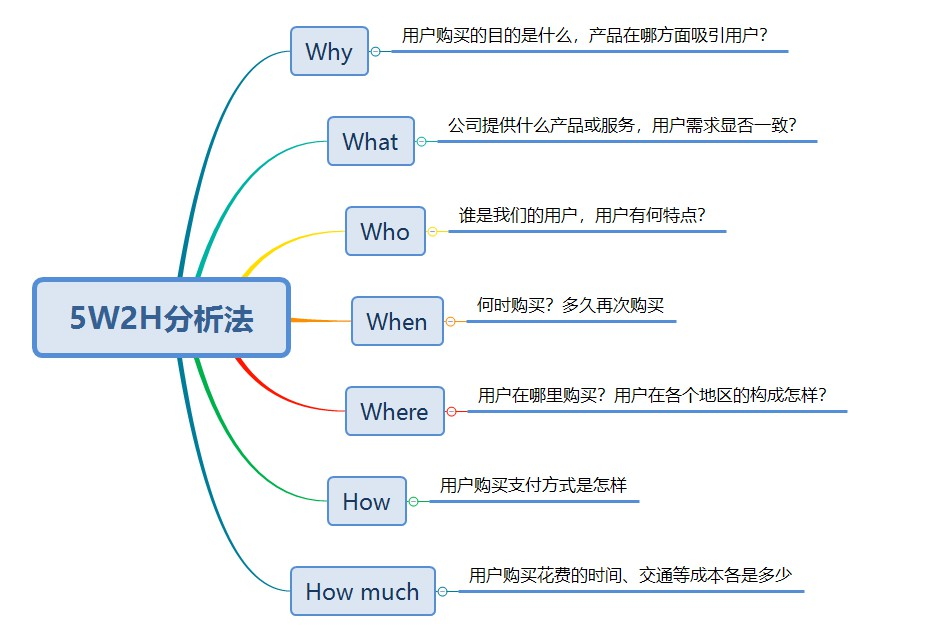
\includegraphics[width=5in]{example/5W2H.JPG}
\caption{5W2H分析法在用户购买行为分析上的应用}
\label{fig:1-2}
%\end{minipage}

\end{figure}

\subsubsection{逻辑树分析法}

逻辑树(可以理解成通过头脑风暴法绘制思维导图)是分析问题最常使用的工具之一,它是将问题的所有子问题分层罗列,从最高层开始,并逐步向下扩展。把一个已知问题当成树干,然后开始考虑这个问题和哪些相关问题有关。每想到一点,就给这个问题所在的树干加一个"树枝",并标明这个"树枝"代表什么问题。

逻辑树的使用必须遵循以下三个原则。
\begin{enumerate}
	\item 要素化:把相同问题总结归纳成要素。
    \item 框架化:将各个要素组织成框架,遵守不重不漏的原则。
    \item 关联化:框架内的各要素保持必要的相互关系,简单而不孤立。
\end{enumerate}
利用逻辑树分析法,同样可以理清分析思路。例如我们需要进行公司利润下降的专题研究,可采用图\href{fig:1-3}{1-3}所示的框架进行数据分析。当然,要根据自己公司的实际情况进行调整,具体问题具体分析。

\begin{figure}[!htp]

\centering
%\begin{minipage}[t]{5in}
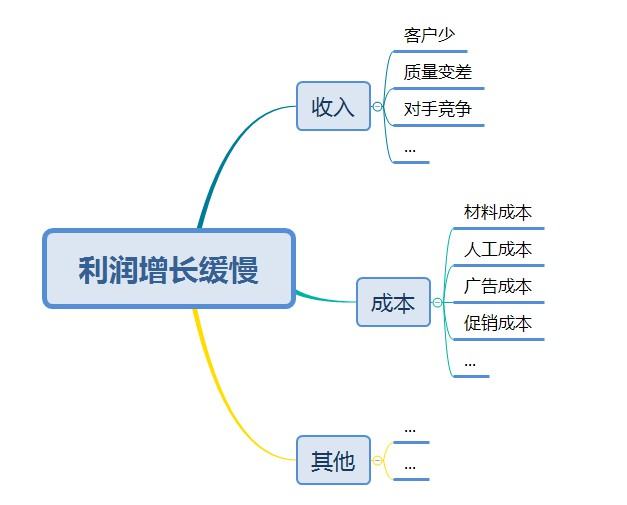
\includegraphics[width=4in]{example/logicTree.JPG}
\caption{逻辑树分析法在利润分析中的应用}
\label{fig:1-3}
%\end{minipage}

\end{figure}

不过逻辑树分析法也有它的缺点,就是涉及的相关问题可能有遗漏,虽然可以用头脑风暴法把涉及的问题总结归纳出来,但还是难以避免存在考虑不周全的地方。所以在使用逻辑树的时候,尽量把涉及的问题或要素考虑周全。

\subsubsection{4P营销理论}

4P营销理论产生于20世纪60年代的美国,它是随着营销组合理论的提出而出现的。营销组合实际上有几十个要素,这些要素可以概括为4 类:产品(Product)、价格(Price)、
渠道(Place)、促销(Promotion),即著名的4P营销理论。

1)产品(Product):从市场营销的角度来看,产品是指能够提供给市场,被人们使用和消费并满足人们某种需要的任何东西,包括有形产品、服务、人员、组织、观念或它们的组合。

2)价格(Price):是指顾客购买产品时的价格,包括基本价格、折扣价格、支付期限等。价格或价格决策关系到企业的利润、成本补偿,以及是否有利于产品销售、促销等问题。
影响定价的主要因素有三个:需求、成本与竞争。最高价格取决于市场需求,最低价格取决于该产品的成本费用,在最高价格和最低价格的幅度内,企业能把这种产品价格定
多高则取决于竞争者的同种产品的价格。

3)渠道(Place):是指产品从生产企业流转到用户手上的全过程中所经历的各个环节。

4)促销(Promotion):是指企业通过销售行为的改变来刺激用户消费,以短期的行为(比如让利,买一送一,营销现场气氛等等)促成消费的增长,吸引其他品牌的用户或
导致提前消费来促进销售的增长。广告、宣传推广、人员推销、销售促进是一个机构促销组合的四大要素。

如果需要了解公司的整体运营情况,就可以采用4P营销理论对数据分析进行指导,这样就可以为全面地了解到公司的整体运营情况。现在就以4P营销理论为指导,搭建公司业务分析框架,如图\href{fig:1-4}{1-4}所示。

\begin{figure}[!htp]

\centering
%\begin{minipage}[t]{5in}
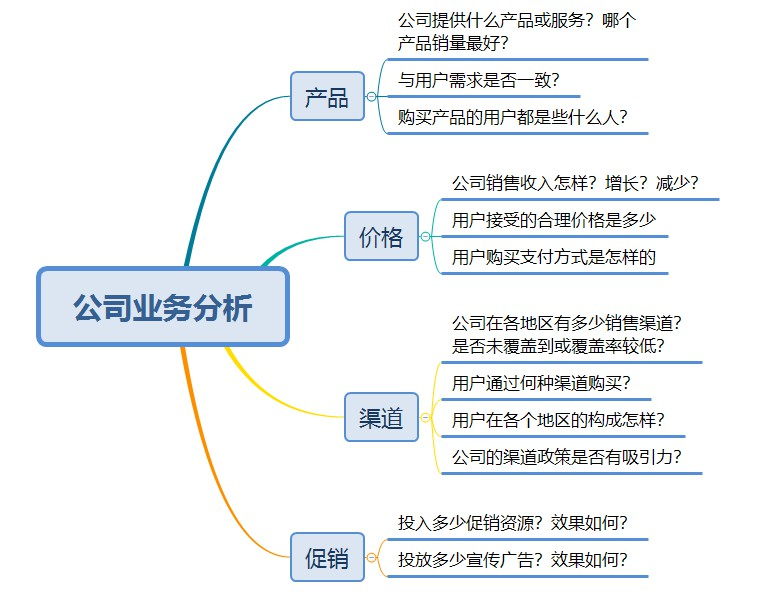
\includegraphics[width=5in]{example/4P.JPG}
\caption{4P营销理论在公司业务分析中的应用}
\label{fig:1-4}
%\end{minipage}

\end{figure}

\subsubsection{用户行为理论}

网站分析的发展已经较为成熟,它有一套成熟的分析指标,比如IP、PV(Page View 访问量)、页面停留时间、跳出率、回访者、新访问者、回访次数、回访相隔天数、流失率、关键字搜索、转化率、登录率,等等。遇到这么多指标,所有的指标都要采用吗?什么指标该采用?什么指标又不该采用?各指标之间有何联系?哪个指标先分析?哪个指标后分析?

因此我们需要梳理这些之间的逻辑关系,比如利用用户使用行为理论进行梳理。用户使用行为是指用户为获取、使用物品或服务所采取的各种行动,用户对产品首先需要有
一个认知、熟悉的过程,然后试用,再决定是否继续消费使用,最后成为忠诚用户。用户使用行为的完整过程,如图\href{fig:1-5}{1-5} 所示。

\begin{figure}[!htp]

\centering
%\begin{minipage}[t]{5in}
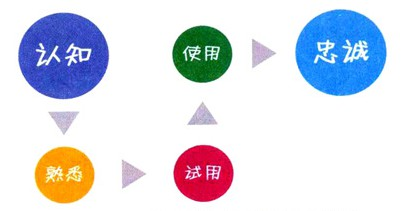
\includegraphics[width=3in]{example/user_behavior.JPG}
\caption{用户使用行为的轨迹示例}
\label{fig:1-5}
%\end{minipage}

\end{figure}

现在我们可利用用户使用行为理论,梳理网站分析的各关键指标之间的逻辑关系,构建符合公司实际业务的网站分析指标体系,如图\href{fig:1-6}{1-6}所示。 \\

\begin{figure}[!htp]

\centering
%\begin{minipage}[t]{5in}
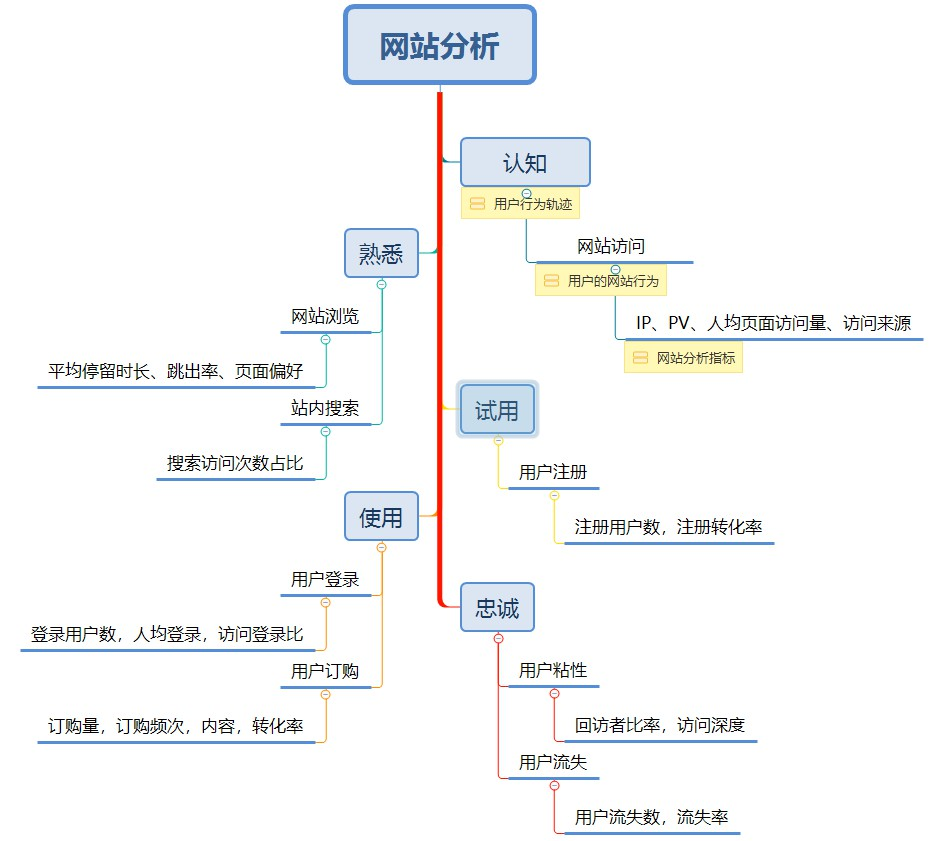
\includegraphics[width=5in]{example/user_behavior1.JPG}
\caption{用户使用行为理论在网站分析中的应用}
\label{fig:1-6}
%\end{minipage}

\end{figure}

对以上的数据分析方法论小总结一下:
\begin{itemize}
	\item PEST分析理论主要用于行业分析。
    \item 4P分析理论主要用于公司整体经营情况分析。
    \item 逻辑树分析理论可用于业务问题专题分析。
    \item 用户行为理论的用途较单一,就是用于用户行为研究分析。
    \item 5W2H分析理论的用途相对广泛,可用于用户行为分析、业务问题专题分析等。
\end{itemize}

\subsection{数据分析方法}

常见的数据分析方法有:对比分析,平均分析,综合评价分析,分组分析,结构分析,交叉分析,杜邦分析,漏斗图分析,矩阵关联分析,聚类分析,回归分析,时间序列分析,决策树,神经网络。数据分析作用及对应的分析方法如表\href{table:1-1}{1-1}所示
\begin{table}[!hpb]
\centering
\caption{数据分析作用及对应的分析方法}
\begin{tabular}{|c|c|l}
\hline
\multicolumn{1}{|l|}{数据分析作用} & \multicolumn{1}{l|}{基本方法} & \multicolumn{1}{l|}{数据分析方法} \\ \hline
\multirow{4}{*}{现状分析}        & \multirow{4}{*}{对比}       & \multicolumn{1}{l|}{对比分析}   \\ \cline{3-3}
                             &                           & \multicolumn{1}{l|}{平均分析}   \\ \cline{3-3}
                             &                           & \multicolumn{1}{l|}{综合评价分析} \\ \cline{3-3}
                             &                           & \multicolumn{1}{l|}{...}    \\ \hline
\multirow{8}{*}{原因分析}        & \multirow{8}{*}{细分}       & \multicolumn{1}{l|}{分组分析}   \\ \cline{3-3}
                             &                           & \multicolumn{1}{l|}{结构分析}   \\ \cline{3-3}
                             &                           & \multicolumn{1}{l|}{交叉分析}   \\ \cline{3-3}
                             &                           & \multicolumn{1}{l|}{杜邦分析}   \\ \cline{3-3}
                             &                           & \multicolumn{1}{l|}{漏斗图分析}  \\ \cline{3-3}
                             &                           & \multicolumn{1}{l|}{矩阵关联分析} \\ \cline{3-3}
                             &                           & \multicolumn{1}{l|}{聚类分析}   \\ \cline{3-3}
                             &                           & \multicolumn{1}{l|}{...}    \\ \hline
\multirow{5}{*}{预测分析}        & \multirow{5}{*}{预测}       & \multicolumn{1}{l|}{回归分析}   \\ \cline{3-3}
                             &                           & \multicolumn{1}{l|}{时间序列}   \\ \cline{3-3}
                             &                           & \multicolumn{1}{l|}{决策树}    \\ \cline{3-3}
                             &                           & \multicolumn{1}{l|}{神经网络}  \\ \cline{3-3}
                             &                           & \multicolumn{1}{l|}{...}    \\ \hline
\end{tabular}
\label{table:1-1}
\end{table}

\subsubsection{对比分析法}

1、定义

所谓对比分析法,是指将两个或两个以上的数据进行比较,分析它们的差异,从而揭示这些数据所代表的事物发展变化情况和规律性。对比分析法的特点是:可以非常直观地看出事物某方面的变化或差距,并且可以准确、量化地表示出这种变化或差距是多少。

2、分类

对比分析法可分为静态比较和动态比较两类:
\begin{itemize}
	\item 静态比较是在同一时间条件下对不同总体指标的比较,如不同部门、不同地区、不同国家的比较,也叫横向比较,简称横比。
    \item 动态比较是在同一总体条件下对不同时期指标数值的比较,也叫纵向比较,简称纵比。
\end{itemize}

这两种方法既可单独使用,也可结合使用。进行对比分析时,可以单独使用总量指标、相对指标或平均指标,也可将它们结合起来进行对比。比较的结果可用相对数表示,如百分数、倍数等指标。

3、注意事项

进行对比分析时还要考虑到以下几点因素:
\begin{itemize}
    \item 指标的口径范围、计算方法、计量单位必须一致,即要用同一种单位或标准去衡量。如果各指标的口径范围不一致,必须进行调整之后才能进行对比。没有统一的标准,就无法比较,或者无法确认比较的结果。例如600美元与3000元人民币就无法直接比较,需要根据当期的汇率进行换算后才可进行比较,否则不具有可比性。
    \item 对比的对象要有可比性。例如不能拿广州市与华西村、大象与蚂蚁、美国与亚洲进行对比。总之,对比对象之间相似之处越多,越具有可比性。因此,我们在选择和确定对比对象时,一定要分析它们是否具有对比的意义。
    \item 对比的指标类型必须一致。无论绝对数指标、相对数指标、平均数指标,还是其他不同类型的指标,在进行对比时,双方必须统一。例如,2010年广州的GDP值与2010年深圳GDP增长率是无法进行对比的,因为这两个指标类型不同。
\end{itemize}

\subsubsection{分组分析法}

1、定义

作数据分析不仅要对总体的数量特征和数量关系进行分析,还要深入总体的内部进行分组分析。分组分析法是一种重要的数据分析方法,这种方法是根据数据分析对象的特征,按照一定的标志(指标),把数据分析对象划分为不同的部分和类型来进行研究,以揭示其内在的联系和规律性。

分组的目的就是为了便于对比,把总体中具有不同性质的对象区分开,把性质相同的对象合并在一起,保持各组内对象属性的一致性、组与组之间属性的差异性,以便进一步运用各种数据分析方法来解构内在的数量关系,因此分组法必须与对比法结合运用。

分组分析法的关键在于确定组数与组距。在数据分组中,各组之间的取值界限称为组限,一个组的最小值称为下限,最大值称为上限;上限与下限的差值称为组距;上限值与下限值的平均数称为组中值,它是一组变量值的代表值。


2、分类

分组分析法包括等距分组和不等矩分组分析法:

等距分组步骤如下:
\begin{itemize}
    \item 1) 确定组数。这个可以由数据分析师决定,根据数据本身的特点(数据的大小)来判断确定。由于分组的目的之一是为了观察数据分布的特征,因此确定的组数应适中。如果组数太少,数据的分布就会过于集中,组数太多,数据的分布就会过于分散,这都不便于观察数据分布的特征和规律。
    \item 2) 确定各组的组距。组距是一个组的最大值与最小值之差,可根据全部数据的最大值和最小值及所分的组数来确定,即:组距=(最大值一最小值)/组数
    \item 3) 根据组距大小,对数据进行分组整理,划归至相应组内。
\end{itemize}

分好组后,我们就可以进行相应信息的分组汇总分析,从而对比各个组之间的差异以及与总体间的差异情况。

采用等距分组还是不等距分组,取决于所分析研究对象的性质特点。在各单位数据变动比较均匀的情况下比较适合采用等距分组;在各单位数据变动很不均匀的情况下比较适合采用不等距分组,此时不等距分组或许更能体现现象的本质特征。数据分析师可根据自己需要选择。

\subsubsection{结构分析法}

1、定义

结构分析法是指被分析总体内的各部分与总体之间进行对比的分析方法,即总体内各部分占总体的比例,属于相对指标。一般某部分的比例越大,说明其重要程度越高,对总体的影响越大。例如通过对国民经济的构成分析,可以得到生产、流通、分配和消费各环节占国民经济的比重,或是各部门贡献比重,揭示各部分之间的相互联系及其变化规律。结构相对指标(比例)的计算公式为:
\begin{equation}
\mbox{结构相对指标(比例)}=(\mbox{总体某部分的数值}/\mbox{总体总量}) * 100 \%
\end{equation}

2、例子

结构分析法的优点是简单实用,在实际的企业运营分析中,市场占有率就是一个非常经典的应用。
\begin{equation}
\mbox{市场占有率}=(\mbox{某种商品销售量}/\mbox{该种商品市场销售总量}) * 100 \%
\end{equation}

市场占有率是分析企业在行业中竞争状况的重要指标,也是衡量企业运营状况的综合经济指标。市场占有率高,表明企业运营状况好,竞争能力强,在市场上占据有利地位;反之,则表明企业运营状态差,竞争能力弱,在市场上处于不利地位。

\subsubsection{平均分析法}

1、定义

平均分析法就是运用计算平均数的方法来反映总体在一定时间、地点条件下某一数量特征的一般水平。平均指标可用于同一现象在不同地区、不同部门或单位间的对比,还可用于同一现象在不同时间的对比。
平均指标有算术平均数、调和平均数、几何平均数、众数和中位数等,其中最为常用的是算术平均数,也就是日常所说的平均数或平均值。
算术平均数的计算公式为:
\begin{equation}
\mbox{算术平均数}=(\mbox{总体各单位数值的总和}/\mbox{总体单位个数}) * 100 \%
\end{equation}

2、作用

平均分析法的主要作用有两点:
\begin{itemize}
    \item 利用平均指标对比同类现象在不同地区、不同行业、不同类型单位等之间的差异程度,比用总量指标对比更具有说服力。
    \item 利用平均指标对比某些现象在不同历史时期的变化,更能说明其发展趋势和规律。
\end{itemize}

算术平均数是非常重要的基础性指标。平均数是综合指标,它的特点是将总体内各单位的数量差异抽象化,它只能代表总体的一般水平,掩盖了在平均数后各单位的差异。
平均分析法要结合各种分组和指标对比来进行。比如分析不同行业、地区的平均从业人数、平均营业收入等。总之,对于所有数量指标都可以依据不同的分组用单位数来平均,进行对比与分析。

\subsubsection{交叉分析法}

1、定义

交叉分析法通常用于分析两个变量(字段)之间的关系,即同时将两个有一定联系的变量及其值交叉排列在一张表格内,使各变量值成为不同变量的交叉结点,形成交叉表,从而分析交叉表中变量之间的关系,所以也叫交叉表分析法。交叉表当然也有二维以上的,维度越多,交叉表就越复杂,所以在选择几个维度的时候需要根据分析的目的决定。

2、例子

假设A,B,C三个地区销售三种水果,通过下面的二维交叉表,我们可以分析不同地区,不同水果的具体销售情况。
\begin{table}[]
\centering
\caption{二月各地区水果销量交叉表示例}
\begin{tabular}{|l|l|l|l|l|}
\hline
地区  & 苹果  & 桃子                        & 鸭梨  & 行小计 \\ \hline
A   & 73  & {\color[HTML]{333333} 64} & 72  & 209 \\ \hline
B   & 70  & 63                        & 56  & 189 \\ \hline
C   & 69  & 48                        & 68  & 185 \\ \hline
列小计 & 212 & 175                       & 196 & 583 \\ \hline
\end{tabular}
\end{table}

\begin{itemize}
    \item 一、二月份所有地区所有水果的总销量(总计)。
    \item 一、二月份不同地区所有水果的销量(行小计)。
    \item 一、二月份不同水果所有地区的销量(列小计)。
    \item 一、二月份各个地区不同水果的销量(各交叉结点值)。
\end{itemize}

\subsubsection{综合评价分析法}

1、定义

前面介绍的对比分析法,分组分析法,结构分析法,平均分析法,交叉表分析法,这些都是简单分析法,对于分析简单的对象没有问题。但是随着数据分析的广泛开展,分析评价的对象越来越复杂,简单分析法的局限性也越来越明显。经常会出现从这几个指标看甲单位优于乙单位,从那几个指标看乙单位优于丙单位,从其他指标看丙单位又优于甲单位的情况,使分析者难以评价到底熟优熟劣。

因此,人们通过对实践活动的总结,逐步形成了一系列运用多个指标对多个参评单位进行评价的方法,称为多变量综合评价分析方法,简称综合评价分析法。综合评价分析法的基本思想是将多个指标转化为一个能够反映综合情况的指标来进行分析评价,比如不同国家的经济实力,不同地区的社会发展水平,小康生活水平达标进程,企业经济效
益评价等,都可以应用这种方法。

2、步骤
\begin{itemize}
    \item 1) 确定综合评价指标体系,即包含哪些指标,是综合评价的基础和依据。
    \item 2) 收集数据,并对不同计量单位的指标数据进行标准化处理(0-1标准化,Z标准化)\footnote{标准化和归一化什么区别? \quad \url{
https://www.zhihu.com/question/20467170/answer/633379185}} 。
    \item 3) 确定指标体系中各指标的权重,以保证评价的科学性。
    \item 4) 对经处理后的指标再进行汇总计算出综合评价指数或综合评价分值。
    \item 5) 根据评价指数或分值对参评单位进行排序,并由此得出结论。
\end{itemize}

其中各指标权重的确定,是综合评价分析方法中较为关键的一步。确定指标权重的方法较多,比如专家访谈法、德尔菲法、层次分析法、主成分分析法、因子分析法、回归分析法等,这些方法都较为复杂,操作起来也相对困难,这里介绍一种比较简单的权重确定法,即目标优化矩阵表。

目标优化矩阵的工作原理就是把人脑的模糊思维,简化为计算机的$1/0$式逻辑思维,最后得出量化的结果,这种方法不仅量化准确,而且简单、方便、快捷。目标优化矩阵的用途是非常广泛的,它不但可以用于目标的优化,还可以用于任何项目的排序,如重要性排序等。对于目标优化矩阵中涉及的权重数值,可以找几个有经验或专业的人士,通过他们的投票表决来确定各项的重要性,从而获知各项目的权重数值。

目标优化矩阵表的用法为:将纵轴上的项目依次与横轴上的项目对比,由专家进行投票表决,如果纵轴上的项目比横轴上的项目重要,那么在两个项目相交的格子中填“1”,否则填“0”,最后将每行数字相加,根据合计的数值进行排序。下面通过一个例子来理解该方法。

3、实例

假设对人才评价的指标有4个:人品、动手能力、创新意识、教育背景,公司HR需要对每个应试者打分,并计算综合得分,现在需要确定这4个指标的权重,此时我们就可以利用目标优化矩阵表,如表\href{}{}所示。从纵轴的“人品”指标开始,与横轴的“人品”“动手能力”“创新意识”“教育背景”这四个指标逐一进行比较:
\begin{itemize}
    \item 1) 用“人品”对比“动手能力”,假设“人品”没“动手能力”重要,输入“0”。
    \item 2) 用“人品”对比“创新意识”,假设“人品”比“创新意识”重要,输入“1”。
    \item 3) 用“人品”对比“教育背景”,假设“人品”比“教育背景”重要,输入“1”。。
\end{itemize}

因此,某指标权重计算公式如下:
\begin{equation}
\mbox{某指标权重}=(\mbox{某指标重要性合计得分}/\mbox{所有指标重要性合计得分}) * 100 \%
\end{equation}

\begin{table}[]
\centering
\caption{人才评价综合指标的目标优化矩阵表}
\begin{tabular}{|l|l|l|l|l|l|l|}
\hline
人才评价 & 人品               & 动手能力                     & 创新意识             & 教育背景             & 合计 & 排序 \\ \hline
人品   & \textbackslash{} & {\color[HTML]{333333} 0} & 1                & 1                & 2  & 2  \\ \hline
动手能力 & 1                & \textbackslash{}         & 1                & 1                & 3  & 1  \\ \hline
创新意识 & 0                & 0                        & \textbackslash{} & 1                & 1  & 3  \\ \hline
教育背景 & 0                & 0                        & 0                & \textbackslash{} & 0  & 4  \\ \hline
\end{tabular}
\end{table}

在NBA球员数据分析中,球员的努力因子(EFF)作为一种综合分析指标,也是通过结合多种指标(PTS,REB,BLK,STL,TOV等)加权计算得到的,如图\href{figure:1-7}{1-3}所示 \footnote{\url{https://www.nba.com/stats/leaders/}}。

\begin{figure}[!htp]

\centering
%\begin{minipage}[t]{5in}
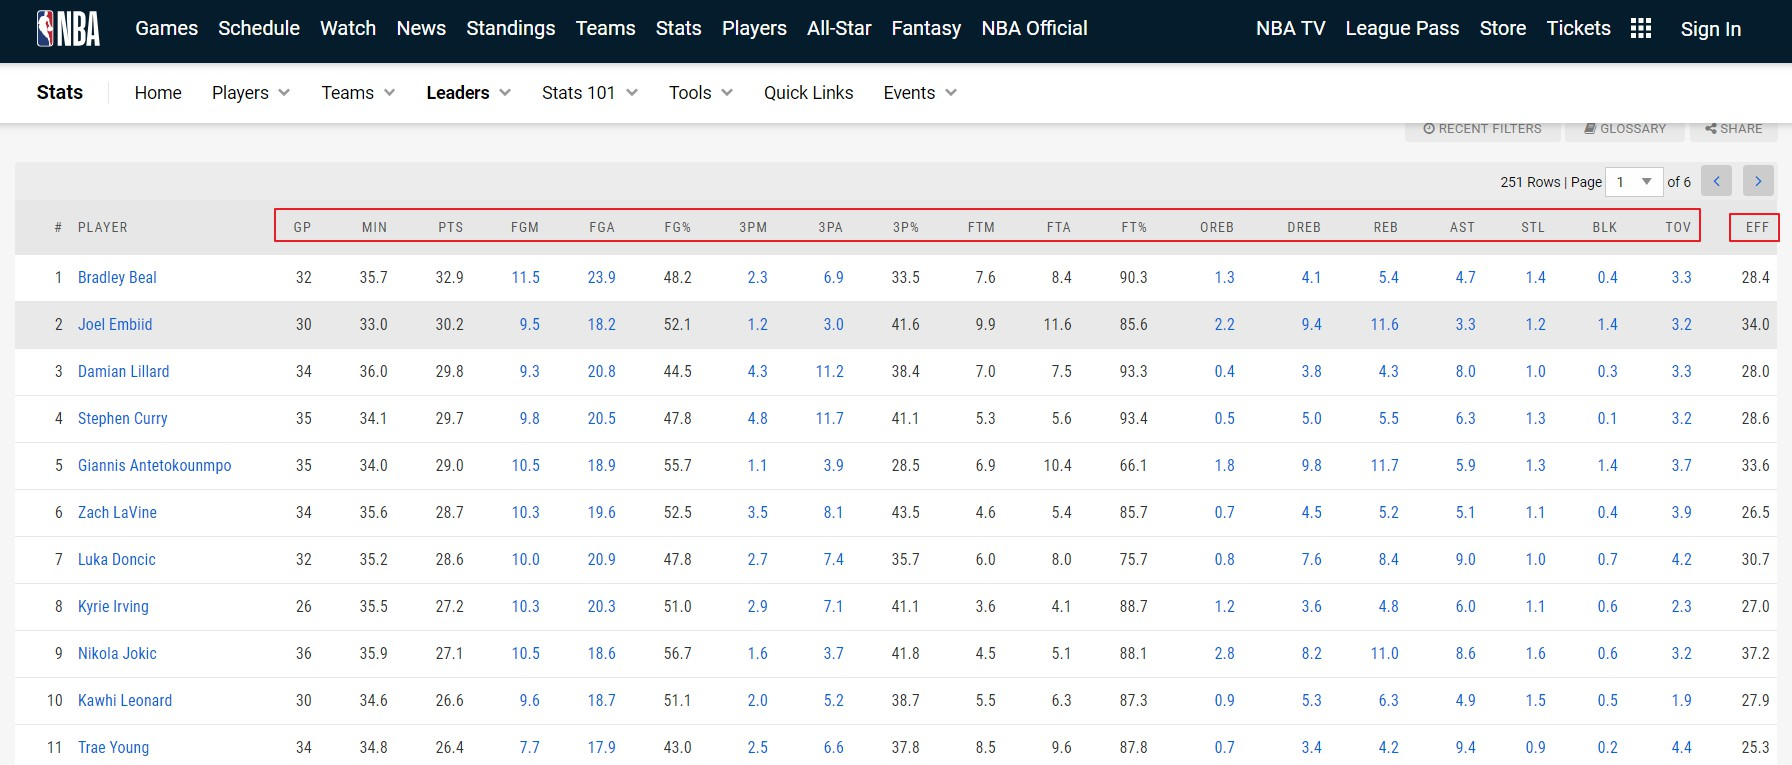
\includegraphics[width=5.5in]{example/nba.JPG}
\caption{EFF因子}
\label{figure:1-7}
%\end{minipage}

\end{figure}

\subsubsection{杜邦分析法}

1、定义

杜邦分析法是由美国杜邦公司创造并最先采用的一种综合分析方法,又称杜邦财务分析体系,简称杜邦体系。它是利用各主要财务指标间的内在联系,对企业财务状况及经济效益进行综合分析评价的方法。

该体系以净资产收益率为龙头,如图\href{}{}所示,以总资产收益率和权益乘数为核心,重点揭示企业盈利能力及权益乘数对净资产收益率的影响,以及各相关指标间的相互影响关系,为各级管理者优化经营理财状况、提高公司经营效益提供了思路。提高总资产收益率的根本在于扩大销售、节约成本、优化投资配置、加速资金周转、优化资金结构、确定风险意识等。

\begin{figure}[!htp]

\centering
%\begin{minipage}[t]{5in}
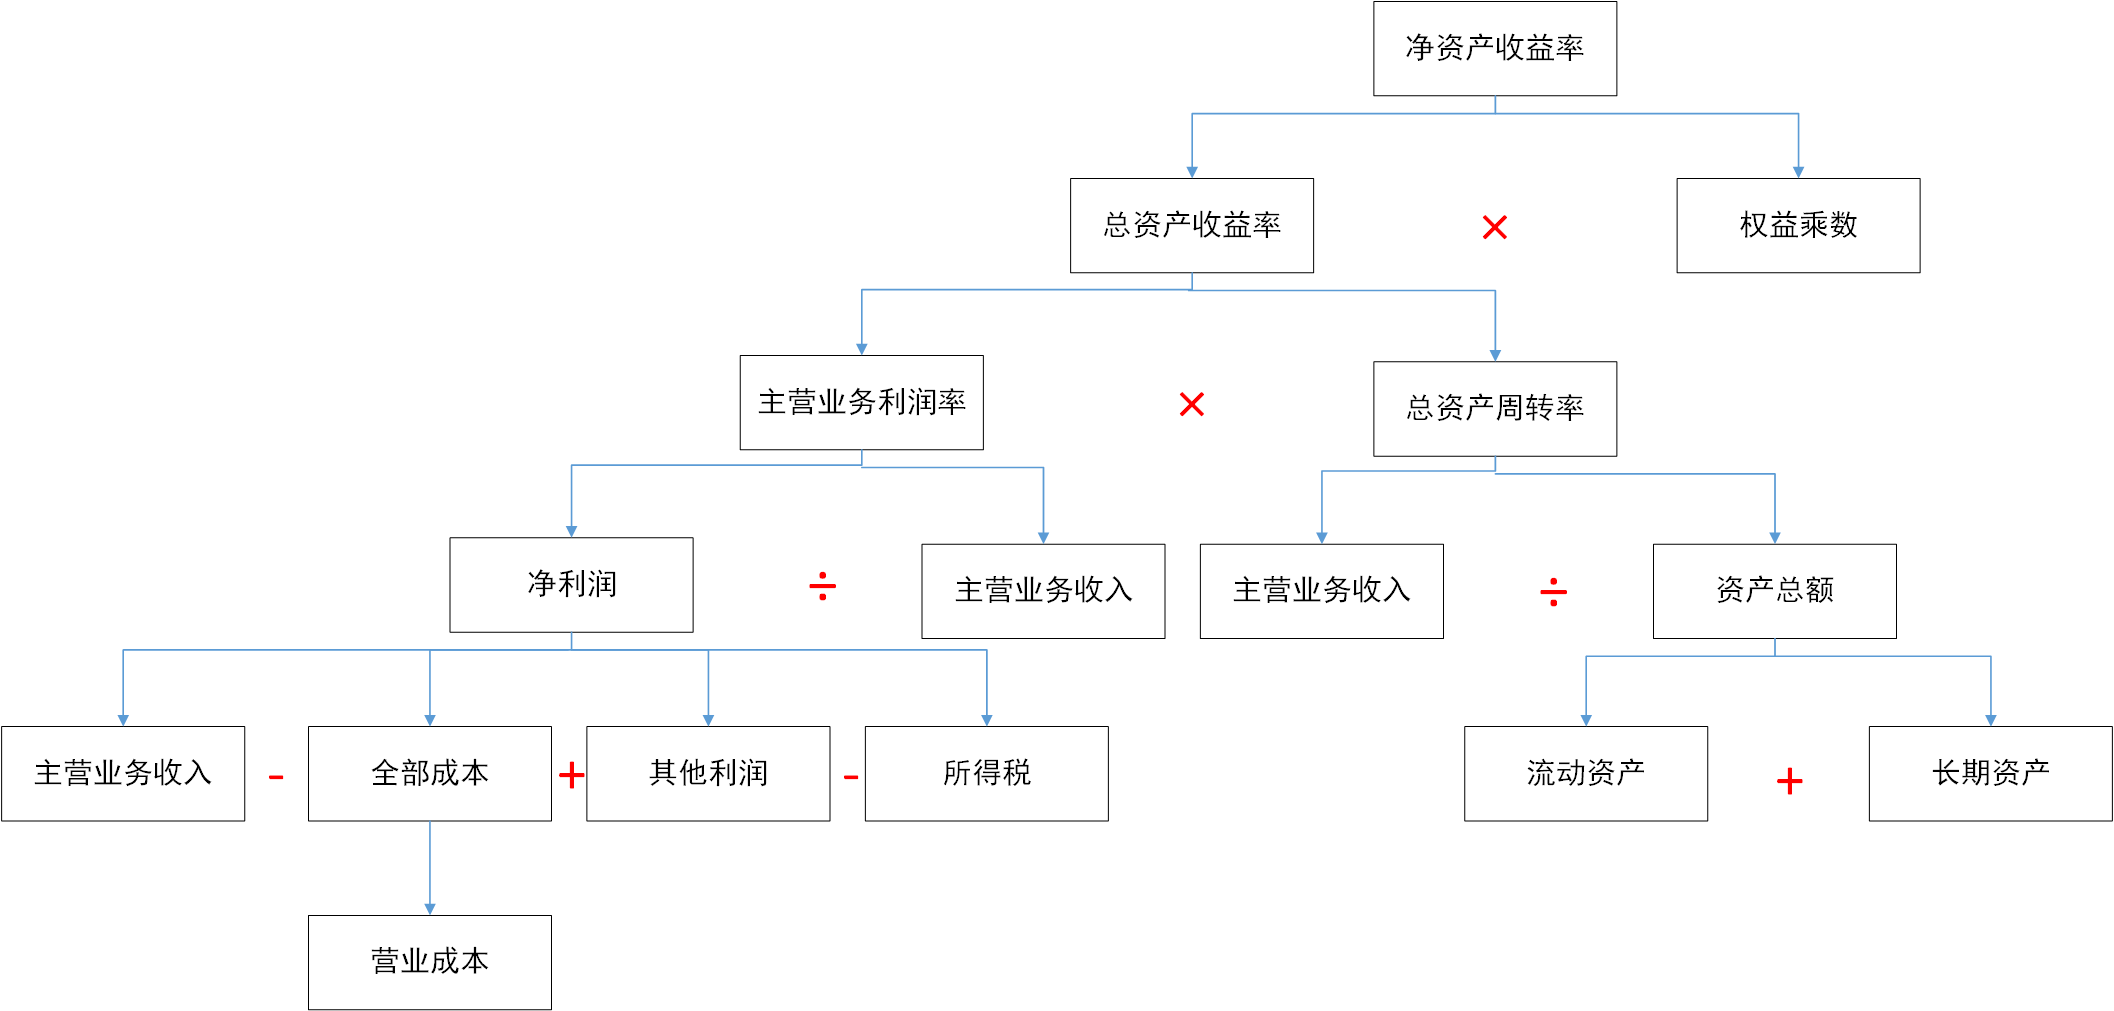
\includegraphics[width=5.5in]{example/dubang.png}
\caption{杜邦分析法}
\label{figure:1-7}
%\end{minipage}

\end{figure}

杜邦分析体系的特点是,将若干个用以评价企业经营效率和财务状况的比率按其内在联系有机地结合起来,形成一个完整的指标体系,并最终通过权益收益率来综合反映。
杜邦分析采用金字塔形结构,自顶向下逐层分析原因,使财务比率分析的层次更清晰、条理更突出,简洁明了地表达了各财务指标之间的关系。

2、实例

不光是利润率下降的问题,如果遇到其他类似问题,都可以采用杜邦分析法。虽然杜邦分析法主要用于财务方面的分析,但可以利用这种方法结合我们的业务进行分析。例如现有某行业A公司2020年的市场占有率同比下降7$\%$ \footnote{环比与同比 \quad \url{https://zhidao.baidu.com/question/581528234.html}},但公司的用户规模在增长,老板问你原因何在?这时我们就可以采用杜邦分析方法逐层查找原因,如图\href{}{} 所示。

\begin{figure}[!htp]

\centering
%\begin{minipage}[t]{5in}
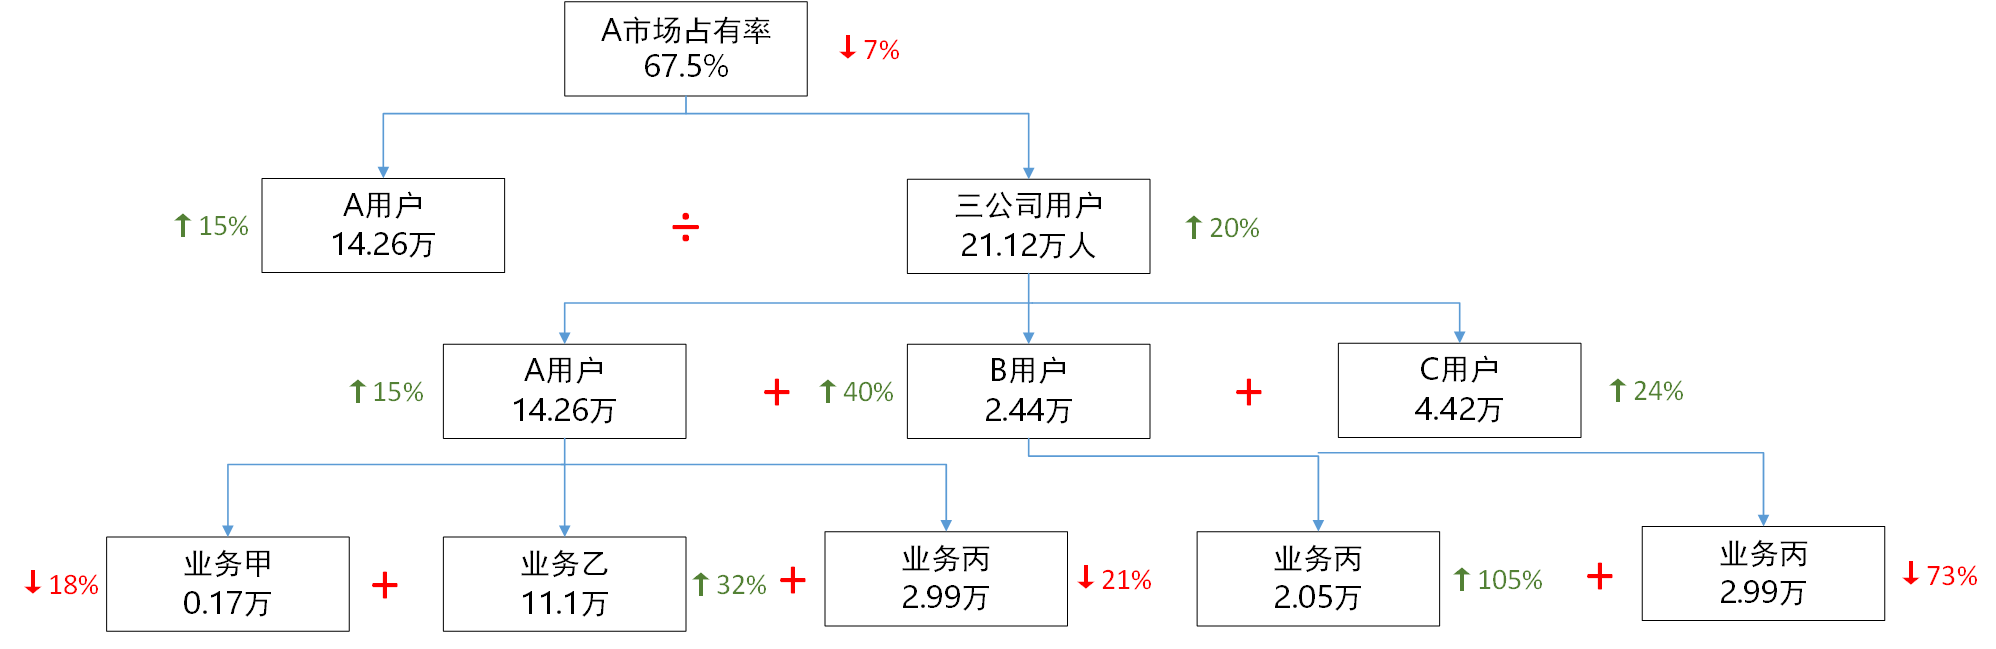
\includegraphics[width=6in]{example/dubang1.png}
\caption{利用杜邦分析法分析市场占有率下降示例}
\label{figure:1-7}
%\end{minipage}

\end{figure}

通过杜邦分析,我们可发现A公司2020年市场占有率不降的主要原因:
\begin{itemize}
    \item B公司的业务丁与2019年相比有大幅增长,拉动B公司用户的增长。
    \item C公司的用户与2019年相比也有一定幅度的增长。
    \item A公司用户与2019年相比虽然也有15$\%$的增长,但是与B、C公司相比,A公司用户增长幅度相对较小,从而使A公司的市场占有率比2019年下降7$\%$。
    \item 我们还可发现A公司业务甲和业务丙与2019年相比都在下降,而A公司的用户增长主要由业务乙拉动。
\end{itemize}

\subsubsection{漏斗图分析法}

1、定义

漏斗图是一个适合业务流程比较规范、周期比较长、各流程环节涉及复杂业务过程比较多的管理分析工具。为什么要在分析业务流程的时候使用漏斗图?因为漏斗图是对业务流程最直观的一种表现形式,并且也最能说明问题的所在。通过漏斗图可以很快发现业务流程中存在问题的环节。例如漏斗图用于网站中某些关键路径的转化率的分析,不仅能显示用户从进入网站到实现购买的最终转化率,同时还可以展示整个关键路径中每一步的转化率,如图所示。

\begin{figure}[!htp]

\centering
%\begin{minipage}[t]{5in}
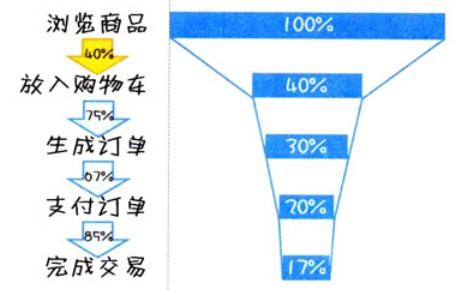
\includegraphics[width=3in]{example/loudou.JPG}
\caption{使用漏斗图分析用户在业务中的转化率和流失率}
\label{figure:1-7}
%\end{minipage}

\end{figure}

单一的漏斗图无法评价网站某个关键流程中各步骤转化率的好坏。我们可以利用之前介绍的对比分析方法,对同一环节优化前后的效果进行对比分析,或对同一环节不同细分用户群的转化率作比较,或对同行业类似产品的转化率进行对比,等等。

2、作用

漏斗图不仅能告诉我们用户在业务中的转化率和流失率,还可以告诉我们各种业务在网站中的受欢迎程度或重要程度。通过对不同业务的漏斗图进行对比,可以找出何种业务在网站中更受用户的欢迎或更吸引用户。只要你掌握了之前介绍的对比分析方法,就可以从不同业务角度发现隐藏在其中的业务问题。

\subsubsection{矩阵关联分析法}

1、定义

矩阵分析法是指根据事物(如产品、服务等)的两个重要属性(指标)作为分析的依据,进行分类关联分析,找出解决问题的一种分析方法,也称为矩阵关联分析法,简称矩阵分析法。

\begin{figure}[!htp]

\centering
%\begin{minipage}[t]{5in}
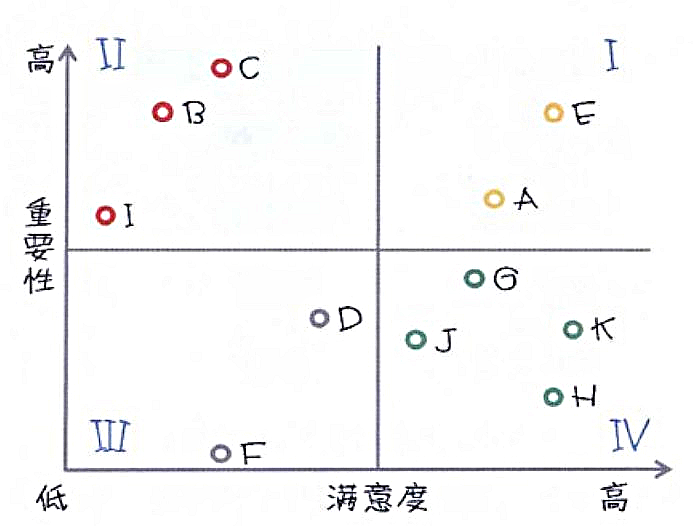
\includegraphics[width=4in]{example/matrix.png}
\caption{2020年某公司用户满意度优先改进矩阵图}
\label{figure:1-11}
%\end{minipage}

\end{figure}

以属性A为横轴,属性B为纵轴,组成一个坐标系,在两坐标轴上分别按某一标准(可取平均值、经验值、行业水平等)进行刻度划分,构成四个象限,将要分析的每个事物对应投射至这四个象限内,进行交叉分类分析,直观地将两个属性的关联性表现出来,进而分析每一个事物在这两个属性上的表现,如图\href{figure:1-11}{1-11}所示,因此它也称为象限图分析法。

矩阵关联分析法在解决问题和资源分配时,为决策者提供重要参考依据。先解决主要矛盾,再解决次要矛盾,有利于提高工作效率,并将资源分配到最能产生绩效的部门、工作中,有利于决策者进行资源优化配置。

2、作用

下面我就用经典案例——用户满意度研究进行矩阵应用的介绍。如图\href{figure:1-11}{1-11}所示,该矩阵为2020年某公司用户满意度调查情况,通过矩阵能够非常直观地看出公司在各方面竞争的优势和劣势分别是什么,从而合理分配公司有限的资源,有针对性地确定公司在管理方面需要提升的重点。所以在满意度研究中,此矩阵可称为优先改进矩阵或资源配置矩阵。从图\href{figure:1-11}{1-11}中可知:

\begin{itemize}
    \item 第一象限(高度关注区)属于重要性高、满意度也高的象限。A、E两个服务项目落在这个象限上。它标志着用户对服务项目的满意度与其重要性成比例,即用户对公司提供某方面服务的满意程度与用户所认为此方面服务的重要程度相符合。对这个象限上的两个服务项目,公司应该继续保持并给予支持。
    \item 第二象限(优先改进区)属于重要性高、但满意度低的象限。B、C、I这三个服务项目落在这个象限上。这个象限标志着改进机会,用户对公司提供某方面服务的满意程度大大低于了他们认为此方面服务的重要程度。公司必须谨慎地确定需要什么类型的改进,用户感觉与事实有时候一致,有时候并不一致,所以必须谨慎地对待。如果确定确实是产品或服务存在问题,则要求进行改进。做好这几项服务项目,可以有效提高用户满意度,为公司赢得竞争优势。
    \item 第三象限(无关紧要区)属于重要性低、满意度也低的象限。D、F这两个服务项目落在这个象限上。这个象限标志着用户对服务项目的满意度与其重要性成比例,也即用户对公司某方面提供服务的满意程度与他们认为此方面服务的重要程度相符合。对这个象限上的两个服务项目,公司应该进一步的关注用户对其期望值的变化。
    \item 第四象限(维持优势区)属于重要性低、满意度高的象限。G、H、J、K这四个服务项目落在这个象限上。这个象限标志着资源过度投入,用户对公司提供某方面服务的满意程度大大超过了他们认为此方面服务的重要程度。公司投入了比用户认可满意的结果更多的时间、资金和资源,如果可能,公司应该把在此区投入的过多的资源转移至其他更重要的产品或服务方面,如第二象限上的B、C、I三个服务项目上。
\end{itemize}

3、注意事项

注意在实际使用矩阵分析法时,切勿生搬硬套,因为每个指标的含义都不一样,有的指标是越大越好,如利润率、市场占有率,而有的指标是越小越好,如用户离网率、折旧率等。

4、衍生的矩阵关联分析方法

1) 发展矩阵

假设我们有2009$\sim$2011年对于公司全部产品的用户满意度数据,我们只需把这三年的数据都绘制在一张矩阵图上,并用箭头把每个服务项目在3年中的变化标注出来,如图\href{figure:1-12}{1-12} 所示。此矩阵在简单的矩阵中增加了发展趋势维度,让读者非常直观地了解到之前每个服务项目在用户评价中处于何种位置,现在处于何种位置,将来又如何发展,非常清晰直观,为决策者进行决策提供了强有力的支撑依据。所以我们可以称该矩阵为发展矩阵。

\begin{figure}[!htp]

\centering
%\begin{minipage}[t]{5in}
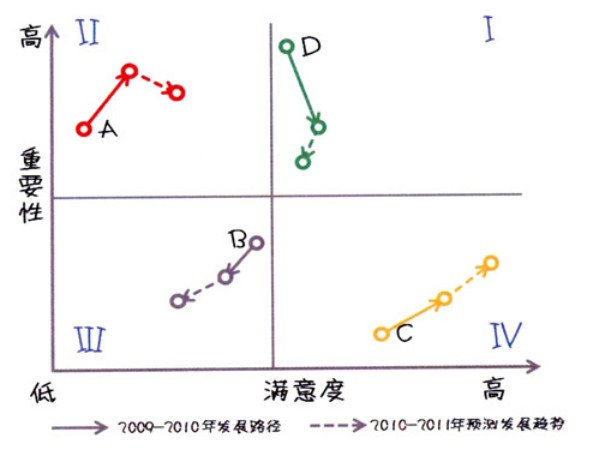
\includegraphics[width=4in]{example/matrix1.jpg}
\caption{发展矩阵示例}
\label{figure:1-12}
%\end{minipage}

\end{figure}

2) 改进难易矩阵

如果企业有较多的短板(需改进的指标)落在图\href{figure:1-11}{1-11}中的第二象限(优先改进区),虽然手心手背都是肉,而企业由于受自身拥有的资源(如人力、物力等)所限,只能先集中有限资源对某个短板进行改进,这时决策者该如何决策把资源投给哪个服务项目呢?其实我们可在原有两个指标的基础上,增加一个指标维度,例如改进难易程度,即企业可以集中有限的资源与精力先改进对企业来说既重要又比较容易改进的短板,如果有足够的资源,再改进相对较难改进的短板,对短板进行逐一击破,从而有效地进行短板的改进。

关于改进的难易程度,这个指标数据并不能直接从用户那里获取,因为用户并不了解,用户只能反映自己对该指标的满意程度。对于这项数据的获取,我们可以采用专家访谈法,获取多位业内专家对各个指标改进难易程度的评价,最后综合各专家的评价以确定最终指标的改进难易程度。另外,也可以用我们之前介绍过的目标优化矩阵来确定难易程度,这与获取权重值的道理一样,通过比较改进的难度来获取其难易程度。

在图\href{figure:1-13}{1-13}这个例子里,图中气泡面积的大小代表着改进难易程度,气泡越大,代表着改进程度越难;气泡越小,代表着改进程度越容易。在改进难易矩阵中可快速准确地确定改进的先后次序,为企业进行短板改进提供有效的决策依据。

\begin{figure}[!htp]

\centering
%\begin{minipage}[t]{5in}
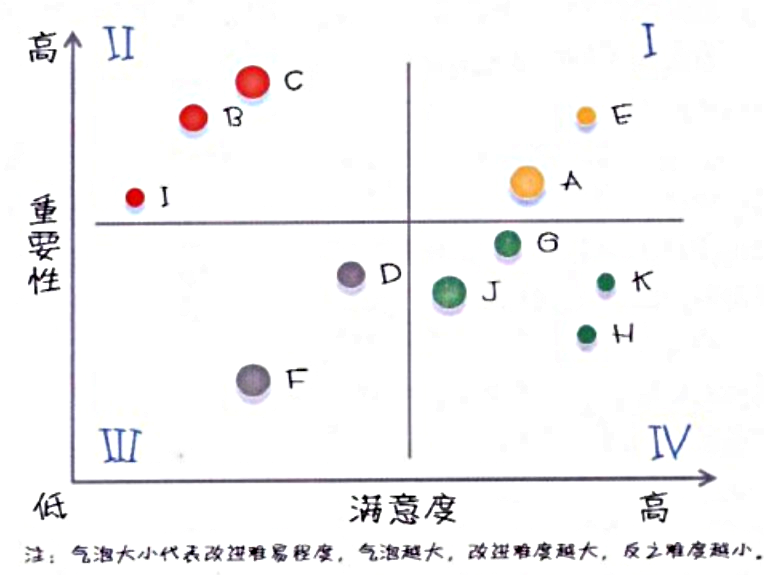
\includegraphics[width=4in]{example/matrix2.png}
\caption{改进难易矩阵示例}
\label{figure:1-13}
%\end{minipage}

\end{figure}

\subsubsection{高级分析方法}

高级分析方法如图\href{figure:1-14}{1-14}所示。

\begin{figure}[!htp]

\centering
%\begin{minipage}[t]{5in}
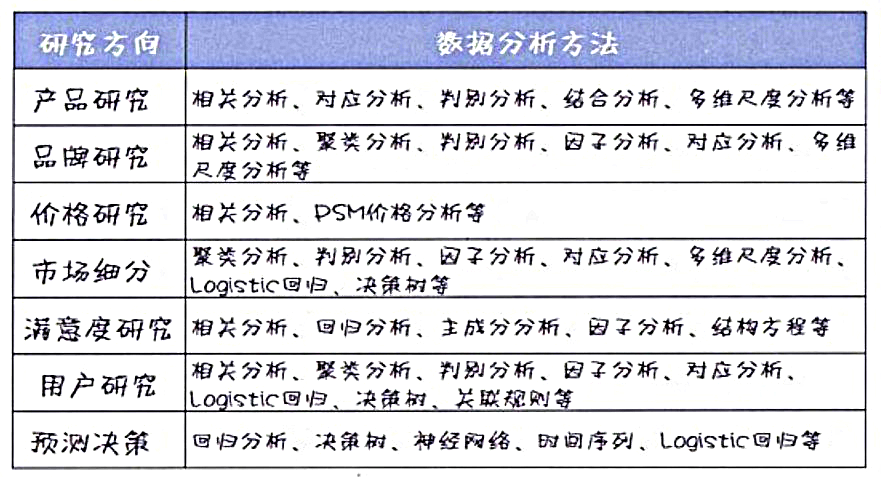
\includegraphics[width=4in]{example/premium.png}
\caption{高级分析方法}
\label{figure:1-13}
%\end{minipage}

\end{figure}

\subsection{数据分析在企业运营分析中的三大误区}

这里主要介绍数据分析在企业运营分析中的三大误区:

1、分析目的不明确,为分析而分析:

对于刚进入数据分析这一行的人来说,经常会问:要用多少图?除了摆数据,还需要说些什么?在此我们应该理解,数据分析不应为了分析而分析,而是应该围绕你的分析目的(了解现状、找出业务变动原因、预测发展等)而进行分析。

只有对自己的目的有清晰的认识,你才知道要怎样去实现这个目的,需要通过哪些图表展现,才会知道这些图表是否能反映问题,自然而然地进行相应的问题分析,而不是连该说些什么都不知道。

2、缺乏业务知识,分析结果偏离实际:

目前现有的数据分析师大多是统计学、计算机、数学等专业出身,他们大多缺乏从事营销、管理方面的工作经验,对业务的理解相对较浅,对数据的分析偏重于数据分析方法的使用,如回归分析、相关分析等。

有的公司老板抱怨手下的数据分析师每天给他看几十个零散数据,虽然做出的报告很专业,图表也很漂亮,但所作的分析忽视了业务逻辑上的关联性,得不到全面、综合性的结论。

在企业中所作的数据分析不是纯数据分析,而是需要多从业务方面进行分析,不应停留在数据表面,要思考数据背后的事实与真相,使得分析结果更加切合实际,为老板的决策提供有力的支撑,否则就是纸上谈兵。

所以说,数据分析师的任务不是单纯做数学题,数据分析师还必须懂营销,懂管理,更要懂策略。

3、一味追求使用高级分析方法,热衷研究模型

在进行数据分析时,相当一部分人都喜欢用回归分析、因子分析等高级分析方法,总认为有分析模型就是专业的,只有这样才能体现专业性,结果才是可信的。其实不然,高级的数据分析方法不一定是最好的,能够简单有效解决问题的方法才是最好的。我们坚信,仅有分析模型远远不够,围绕业务发现问题并解决问题才是数据分析的最终目
的!不论高级的分析方法还是简单的分析方法,只要能够解决业务问题,就是好方法。

\section{机器学习}

人工智能是指使机器像人一样去决策,机器学习是实现人工智能的一种技术,换句话说,机器学习只是人工智能一部分,人工智能不等价于机器学习。

常见的机器学习算法:
\begin{figure}[!htp]

\centering
%\begin{minipage}[t]{5in}
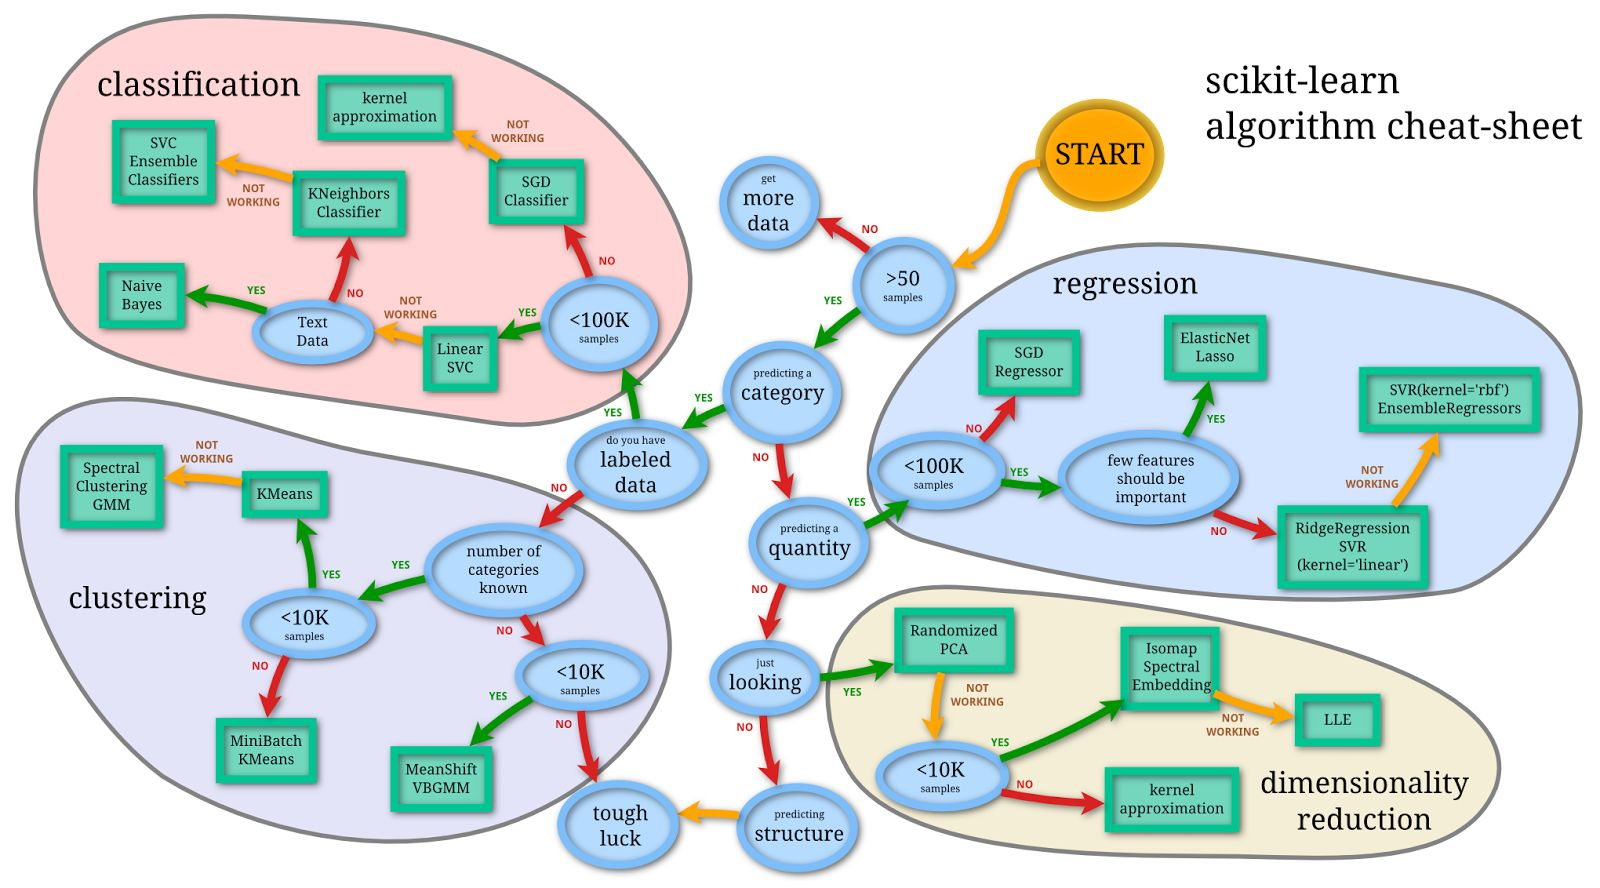
\includegraphics[width=5in]{example/ML_method.JPG}
\caption{常见的机器学习算法}
\label{figure:1-7}
%\end{minipage}

\end{figure}

机器学习、监督学习、无监督学习、深度学习、强化学习关系图如图\href{figure:1-8}{1-8}所示  \footnote{\url{https://book.douban.com/subject/34873001/}}。
\begin{figure}[!htp]

\centering
%\begin{minipage}[t]{5in}
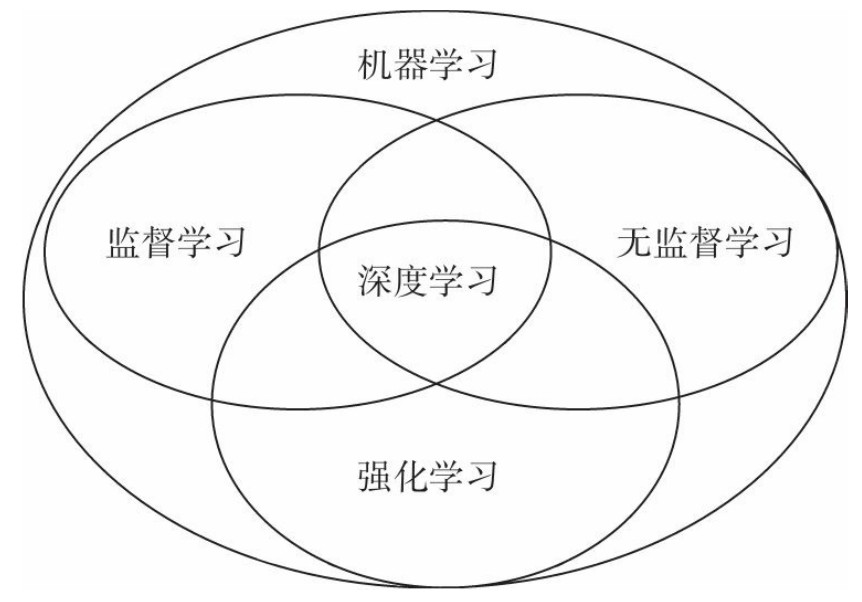
\includegraphics[width=4in]{example/classify1.JPG}
\caption{机器学习、监督学习、强化学习等的关系图}
\label{figure:1-8}
%\end{minipage}
\end{figure}

机器学习一般需要先定义问题、收集数据、探索数据、预处理数据,对数据处理后,接下来开始训练模型、评估模型,然后优化模型等步骤,机器学习一般流程如图\href{figure:1-9}{1-9}所示。

\begin{figure}[!htp]
\centering
%\begin{minipage}[t]{5in}
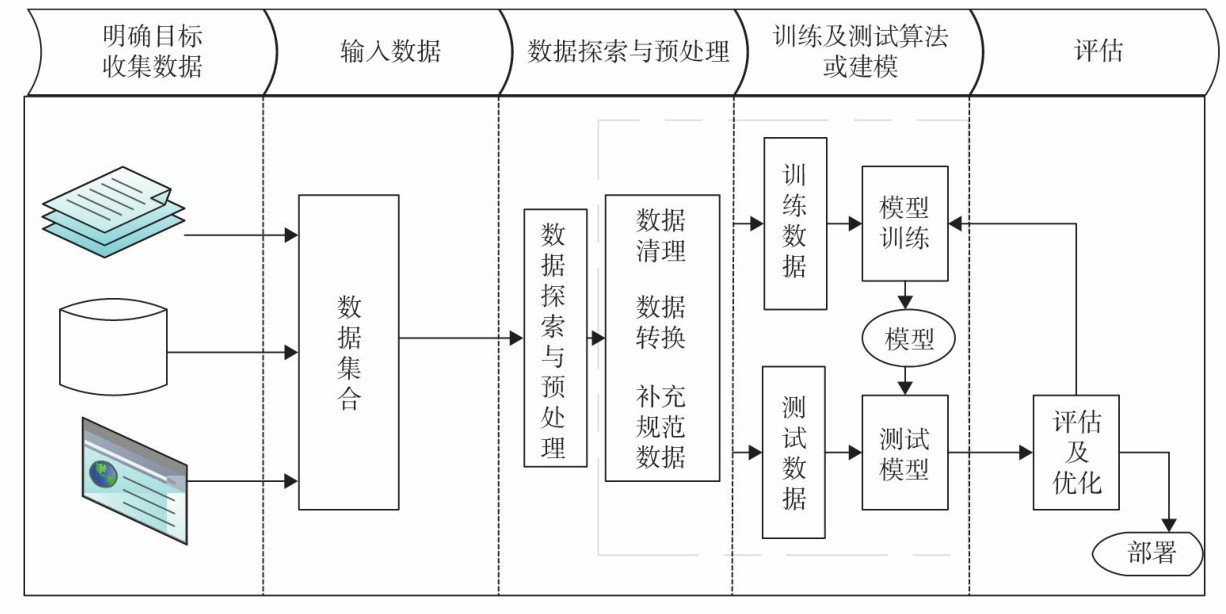
\includegraphics[width=5in]{example/ML1.JPG}
\caption{机机器学习一般流程图}
\label{figure:1-9}
%\end{minipage}
\end{figure}


\subsection{监督学习}

监督学习是最常见的一种机器学习类型,其任务的特点就是给定学习目标,这个学习目标又称标签、标注或实际值等,整个学习过程就是围绕如何使预测与目标更接近而来的。近些年,随着深度学习的发展,分类除传统的二分类、多分类、多标签分类之外,也出现了一些新内容,如目标检测、目标识别、图像分割等监督学习的重要内容。

常见的监督学习算法如图\href{figure:1-10}{1-10}所示。
\begin{figure}[!htp]

\centering
%\begin{minipage}[t]{5in}
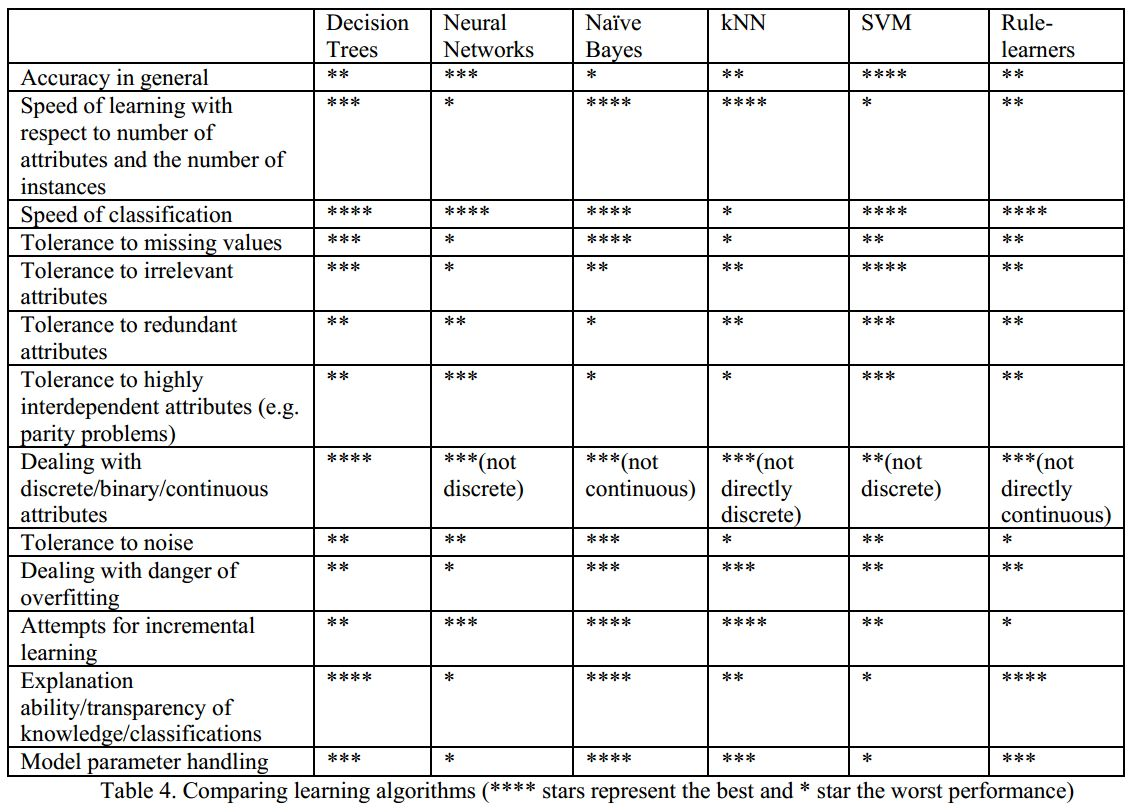
\includegraphics[width=5in]{example/supervised.JPG}
\caption{常见的监督学习算法}
\label{figure:1-9}
%\end{minipage}

\end{figure}

监督学习一般流程如图\href{figure:1-11}{1-11}所示。
\begin{figure}[!htp]
\centering
%\begin{minipage}[t]{5in}
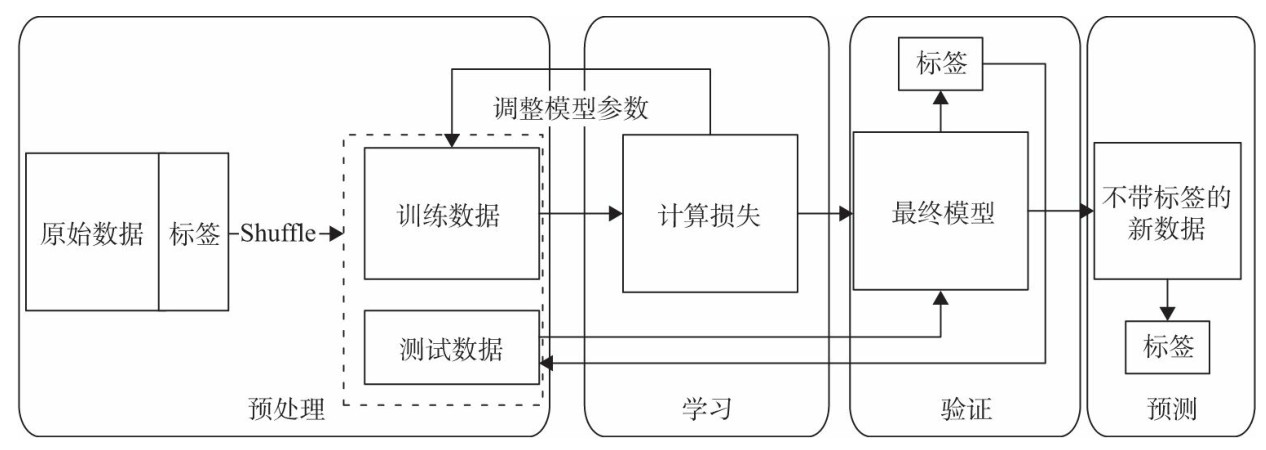
\includegraphics[width=5in]{example/supervisedL.JPG}
\caption{监督学习一般流程}
\label{figure:1-11}
%\end{minipage}
\end{figure}

\subsection{无监督学习}

监督学习的输入数据中有标签或目标值,但在实际生活中,有很多数据是没有标签的,或者标签代价很高。这些没有标签的数据也可能包含很重要的规则或信息,从这类数据中学习到一个规则或规律的过程被称为无监督学习。在无监督学习中,我们通过推断输入数据中的结构来建模,模型包括关联学习、降维、聚类等。

\subsection{半监督学习}

半监督学习是监督学习与无监督学习相结合的一种学习方法。半监督学习使用大量的未标记数据,同时由部分使用标记数据进行模式识别。半监督学习目前正越来越受到人们的重视。

自编码器是一种半监督学习,其生成的目标就是未经修改的输入。语言处理中根据给定文本中的词预测下一个词,也是半监督学习的例子。对抗生成式网络也是一种半监督学习,给定一些真图片或语音,然后通过对抗生成网络生成一些与真图片或是语音逼真的图形或语音。

\subsection{强化学习}

强化学习是机器学习的一个重要分支,是多学科多领域交叉的一个产物。强化学习主要包含4个元素:智能体(Agent)、环境状态、行动和奖励。强化学习的目标就是获得最多的累计奖励。

强化学习把学习看作一个试探评价的过程,Agent选择一个动作用于环境,环境接受该动作后状态发生变化,同时产生一个强化信号(奖或惩)反馈给Agent,Agent根据强化信号和当前环境状态再选择下一个动作,选择的原则是使受到正强化(奖)的概率增大。选择的动作不仅影响立即强化值,也影响下一时刻的状态和最终的强化值。

强化学习不同于监督学习,主要表现在教师信号上。强化学习中由环境提供的强化信号是Agent对所产生动作的好坏做的一种评价,而不是告诉Agent如何去产生正确的动作。由于外部环境只提供了很少的信息,所以Agent必须靠自身的经历进行学习。通过这种方式,Agent在行动一一被评价的环境中获得知识,改进行动方案以适应环境。强化学习大致原理如图\href{figure:1-12}{1-12}所示。

强化学习的特点一般是在探索(exploration)和利用(exploitation)之间进行权衡,“探索”是指系统尝试新类型的动作,“利用”是指系统使用已知能产生较高奖励的动作。过于专注于探索或利用都会产生糟糕的结果\footnote{Pattern Recognition and Machine Learning \quad \url{https://book.douban.com/subject/2061116/}}。

\begin{figure}[!htp]
\centering
%\begin{minipage}[t]{5in}
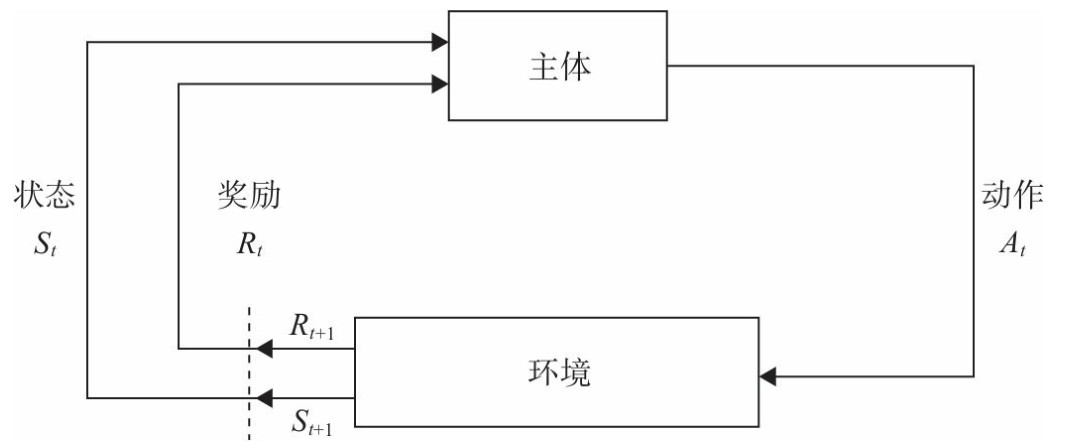
\includegraphics[width=4.5in]{example/RL.JPG}
\caption{强化学习大致原理图}
\label{figure:1-12}
%\end{minipage}
\end{figure}

\subsection{深度学习}


\section{数据分析,机器学习,数据科学三者的区别}

根据数据分析的定义:在杂乱无章的数据中寻找内在规律,我们知道,数据分析无论是在学术界,还是在业界都有应用,但在业界的应用更加广泛和成熟。数据分析专注于在现有的数据集里面,处理和执行统计分析。分析人员集中于创建捕获,处理和组织数据的方法,以发现当前问题的切实可行的见解,并建立呈现此数据的最佳方式。更简单的说,数据分析的领域旨在解决问题,寻求那些我们意识到了问题,但还没找到的问题答案。更重要的是,它的基础是产生可以立即改进的结果。因此,数据分析侧重于使用统计分析等方法解决业务问题,侧重于可解释性分析和数据的可视化,当然为了更好的解决问题也会用到算法模型。输出物一般包括分析报告,统计报表,辅助决策建议等偏重业务决策的结论和分析。

机器学习更侧重于工程和算法研究及应用,主要通过算法和模型解决面向工程和产品化应用的问题,因此输出一般不是具体的可见物,而是工程中核心智能化的部分。

数据科学本质上是应用于数据的计算和统计方法,包括小数据集或大数据集。它也包括诸如探索性数据分析之类的东西,例如对数据进行检查和可视化,以帮助科学家更好地理解数据,并从中做出推论。数据科学还包括诸如数据包装和预处理之类的东西,因此涉及到一定程度的计算机科学,因为它涉及编码和建立数据库、Web服务器之间的连接和流水线等等。

要进行统计,你并不一定得依靠电脑,但如果是数据科学缺了电脑就没法操作了。这就再次说明了虽然数据科学借助统计学,这两者不是一个概念。同理,机器学习也并非人工智能;事实上,机器学习是人工智能的一个分支。这一点挺明显的,因为我们基于以往的数据"教"(训练)机器对特定类型的数据进行概括性的预测。

我的理解是:数据分析也可以使用机器学习模型(比如用到统计学习方法中的boost模型,HMM模型,SVM模型),但是最终的目的是为了绘表做决策,而机器学习的目的是通过 研究算法,提高模型的预测准确度。

表\href{table:1-2}{1-2}简单总结了数据分析,机器学习,数据科学三者的区别。

\begin{table}[!hpb]
\centering
\caption{数据分析,机器学习,数据科学三者的区别}
\resizebox{\textwidth}{15mm}{%
\begin{tabular}{|l|l|l|l|}
\hline
      & 数据分析                & 机器学习            & 数据科学                \\ \hline
范围    & 微观                  & 宏观              & 宏观                  \\ \hline
目的    & 生成报表,辅助决策           & 解决面向工程和产品化应用的问题 & 问正确问题               \\ \hline
主要领域  & 医疗保健,游戏,旅游,即时数据需求工业 & 计算机视觉,自然语言处理等   & 机器学习,AI,搜索引擎工程,企业分析 \\ \hline
使用大数据 & 是                   & 是               & 是                   \\ \hline
\end{tabular}%
}
\label{table:1-2}
\end{table}

读者可以参考引脚给出的链接:数据分析和数据科学的区别\footnote{\url{http://www.360doc.com/content/19/0919/21/410279_862051577.shtml}} \footnote{\url{https://www.sohu.com/a/237669444_401265}}、数据分析和机器学习的区别
\footnote{\url{https://www.zhihu.com/question/65585907/answer/232626359}}、 数据科学的三个职业方向\footnote{\url{https://zhuanlan.zhihu.com/p/26666920}}

\section{统计学习和机器学习的区别}

上面主要介绍了数据分析和机器学习的基本概念,对它们各自的侧重点,我们现在应该有所理解了:数据分析一般使用统计分析方法去研究在杂乱无章数据中的内在规律,目的是为了帮助分析人员绘表并做出合理决策,而机器学习的目的是研究算法和模型,比如研究如何提高其预测准确度,算法鲁棒性等。机器学习是人工智能一个分支,而人工智能的目的是指导机器去做决策,去解决面向工程和产品化应用的问题。

这时笔者有一个疑问,有些时候数据分析也可以使用机器学习模型,比如boost模型,HMM模型和SVM模型,这些模型其实可以归类于统计学习的范畴之中。那么统计学习和机器学习究竟有什么区别?界定在哪?如果我们理解它们之间的界定,对于数据分析和机器学习的界定,我们将会有更深程度的理解。

这里参考\href{https://blog.csdn.net/qq_41892229/article/details/90140493}{统计学和机器学习到底有什么区别?}的解释


\subsection{关于这两个概念的比较分析}
首先,我们必须明白,统计和统计建模是不一样的。统计是对数据的数学研究。除非有数据,否则无法进行统计。统计模型是数据的模型,主要用于推断数据中不同内容的关系,或创建能够预测未来值的模型。通常情况下,这两者是相辅相成的。

因此,实际上我们需要从两方面来论述:第一,统计与机器学习有何不同;第二,统计模型与机器学习有何不同?

说的更直白些就是,有很多统计模型可以做出预测,但预测效果比较差强人意。而机器学习通常会牺牲可解释性以获得强大的预测能力。例如,从线性回归到神经网络,尽管解释性变差,但是预测能力却大幅提高。从宏观角度来看,这是一个很好的答案。至少对大多数人来说已经足够好。然而,在有些情况下,这种说法容易让我们对机器学习和统计建模之间的差异产生误解。让我们看一下线性回归的例子。


或许是因为统计建模和机器学习中使用方法的相似性,使人们认为它们是同一个东西。对这我可以理解,但事实上不是这样。

最明显的例子是线性回归,这可能是造成这种误解的主要原因。线性回归是一种统计方法,通过这种方法我们既可以训练一个线性回归器,又可以通过最小二乘法拟合一个统计回归模型,线性回归模型如图\href{figure:1-7}{1-7}所示。

\begin{figure}[!htp]

\centering
%\begin{minipage}[t]{5in}
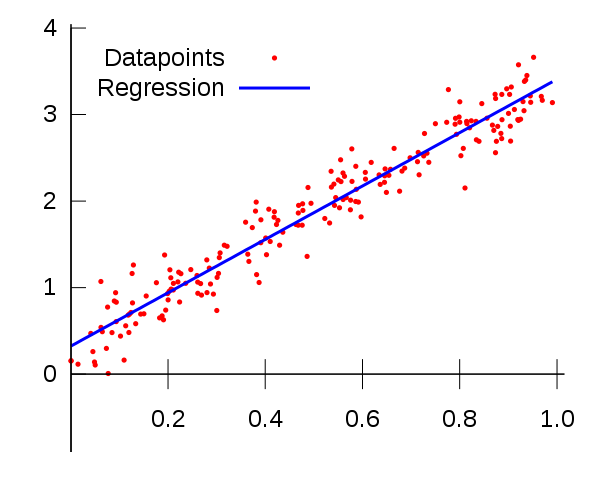
\includegraphics[width=4in]{example/regression.JPG}
\caption{线性回归}
\label{figure:1-7}
%\end{minipage}

\end{figure}

可以看到,在这个案例中,前者做的事儿叫"训练"模型,它只用到了数据的一个子集,而训练得到的模型究竟表现如何需要通过数据的另一个子集测试集测试之后才能知道。在这个例子中,机器学习的最终目的是在测试集上获得最佳性能,使其具有很好的泛化能力。

对于后者,我们则事先假设数据是一个具有高斯噪声的线性回归量,然后试图找到一条线,最大限度地减少了所有数据的均方误差。不需要训练或测试集,在许多情况下,特别是在研究中,建模的目的是描述数据与输出变量之间的关系, 而不是对未来数据进行预测。我们称此过程为统计推断,而不是预测。尽管我们可以使用此模型进行预测,这也可能是你所想的,但评估模型的方法不再是测试集,而是评估模型参数的显著性和健壮性。

机器学习(这里特指有监督学习)的目的是获得一个可反复预测的模型。我们通常不关心模型是否可以解释。机器学习只在乎结果。就好比对公司而言,你的价值只用你的表现来衡量。而统计建模更多的是为了寻找变量之间的关系和确定关系的显著性,恰巧迎合了预测。

如果我试图证明数据变量之间的关系在某种程度上具有统计显著性,以便我可以在科学论文中发表,我将使用统计模型而不是机器学习。这是因为我更关心变量之间的关系,而不是做出预测。做出预测可能仍然很重要,但是大多数机器学习算法缺乏可解释性,这使得很难证明数据中存在的关系。

有一个误解存在了10年:仅基于它们都利用相同的基本概率概念这一事实,来混淆这两个术语是不合理的
而,仅仅基于这两个术语都利用了概率里相同的基本概念这一事实而将他们混为一谈是不合理的。就好比,如果我们仅仅把机器学习当作皮了一层光鲜外衣的统计,我们也可以这样说:

\begin{itemize}
	\item 物理只是数学的一种更好听的说法。
	\item 动物学只是邮票收藏的一种更好听的说法。
	\item 建筑学只是沙堡建筑的一种更好听的说法。
\end{itemize}

这些说法非常荒谬,完全混淆了两个类似想法的术语。

实际上,物理是建立在数学基础上的,理解现实中的物理现象是数学的应用。物理学还包括统计学的各个方面,而现代统计学通常是建立在Zermelo-Frankel集合论与测量理论相结合的框架中,以产生概率空间。它们有很多共同点,因为它们来自相似的起源,并运用相似的思想得出一个逻辑结论。同样,建筑学和沙堡建筑可能有很多共同点,但即使我不是一个建筑师,也不能给出一个清晰的解释,但也看得出它们显然不一样。

在我们进一步讨论之前,需要简要澄清另外两个与机器学习和统计有关的常见误解。这就是数据科学不同于统计学,人工智能不同于机器学习。这些都是没有争议的问题,所以很快就能说清楚。

1)数据科学本质上是应用于数据的计算和统计方法,包括小数据集或大数据集。它也包括诸如探索性数据分析之类的东西,例如对数据进行检查和可视化,以帮助科学家更好地理解数据,并从中做出推论。数据科学还包括诸如数据包装和预处理之类的东西,因此涉及到一定程度的计算机科学,因为它涉及编码和建立数据库、Web服务器之间的连接和流水线等等。要进行统计,你并不一定得依靠电脑,但如果是数据科学缺了电脑就没法操作了。这就再次说明了虽然数据科学借助统计学,这两者不是一个概念。从就业角度来看,想要成为一名数据科学家,需要掌握的知识主要有:编程和数据库、数学和统计、交流和可视化、领导力和软技术技能四个方面。

2)机器学习也并非人工智能;事实上,机器学习是人工智能的一个分支,这一点挺明显的,因为我们基于以往的数据"教"(训练)机器对特定类型的数据进行概括性的预测。为什么这么说呢?因为人工智能(AI)可以分为弱人工智能(ANI)和强人工智能(AGI),我们现在接触到的自动驾驶汽车,智能对话机器人,工厂里的机械臂等都属于ANI的范畴,它是通过以往数据训练学习得到的,而AGI是指高级智能体,他能做任何事情,也许他有自主的思维能力。如果不对AI这么分类,我们很可能局限地认为机器学习就是人工智能,其实不然,人类对人工智能探索的道路还很漫长,只能说现在的机器学习只是实现人工智能终极目标的初级阶段。

\subsection{机器学习是基于统计学}

在我们讨论统计学和机器学习之间的区别前,我们先来说说其相似性,其实文章的前半段已经对此有过一些探讨了。

机器学习基于统计的框架,因为机器学习涉及数据,而数据必须基于统计学框架来进行描述,所以这点十分明显。然而,扩展至针对大量粒子的热力学的统计机制,同样也建立在统计学框架之下。

压力的概念其实是数据,温度也是一种数据。你可能觉得这听起来不合理,但这是真的。这就是为什么你不能描述一个分子的温度或压力,这不合理。温度是分子相撞产生的平均能量的显示。而例如房屋或室外这种拥有大量分子的,我们能用温度来描述也就合理了。

你会认为热力学和统计学是一个东西吗?当然不会,热力学借助统计学来帮助我们理解运动的相互作用以及转移现象中产生的热。

事实上,热力学基于多种学科而非仅仅统计学。类似地,机器学习基于许多其他领域的内容,比如数学和计算机科学。举例来说:

\begin{itemize}
	\item 机器学习的理论来源于数学和统计学。
	\item 机器学习算法基于优化理论、矩阵代数和微积分。
	\item 机器学习的实现来源于计算机科学和工程学概念,比如核映射、特征散列等。
\end{itemize}

\subsection{统计学习理论}

统计学和机器学习之间最主要的区别在于统计学完全基于概率空间。你可以从集合论中推导出全部的统计学内容,集合论讨论了我们如何将数据归类(这些类被称为“集”),然后对这个集进行某种测量保证其总和为1.我们将这种方法成为概率空间。

统计学除了对这些集合和测量有所定义之外没有其他假设。这就是为什么我们对概率空间的定义非常严谨的原因。一个概率空间,其数学符号写作$(\Omega,\Gamma,\rho)$,包含三部分:

\begin{enumerate}
	\item 一个样本空间,$\Omega$,也就是所有可能结果的集合。
	\item 一个事件集合,$\Gamma$,每个事件都包含0或者其它值。
	\item 对每个事件发生的可能性赋予概率,$\rho$,这是一个从事件到概率的函数。
\end{enumerate}

机器学习基于统计学习理论,统计学习理论也依旧基于对概率空间的公理化语言。这个理论基于传统的统计学理论,并发展于19世纪60年代。

统计学习理论中的监督学习,给了我们一个数据集,我们将其标为S= {(xᵢ,yᵢ)},也就是说我们有一个包含N个数据点的数据集,每个数据点由被称为"特征"的其它值描述,这些特征用x描述,这些特征通过特定函数来描绘以返回我们想要的y值。

已知这个数据集,问如何找到将x值映射到y值的函数。我们将所有可能的描述映射过程的函数集合称为假设空间。

为了找到这个函数,我们需要给算法一些方法来"学习"如何最好地着手处理这个问题,而这由一个被称为"损失函数"的概念来提供。因此,对我们所有的每个假设(也即提议的函数),我们要通过比较所有数据下其预期风险的值来衡量这个函数的表现。

预期风险本质上就是损失函数之和乘以数据的概率分布。如果我们知道这个映射的联合概率分布,找到最优函数就很简单了。但是这个联合概率分布通常是未知的,因此我们最好的方式就是猜测一个最优函数,再实证验证损失函数是否得到优化。我们将这种称为实证风险。

之后,我们就可以比较不同函数,找出最小预期风险的那个假设,也就是所有函数中得出最小下确界值的那个假设。

然而,为了最小化损失函数,算法有过度拟合的倾向。这也是为什么要通过训练集"学习"函数,之后在训练集之外的数据集,测试集里对函数进行验证。

如何定义机器学习的本质,我们引出了过度拟合的问题,也对需要区分训练集和测试集作出了解释。而我们在统计学中无需试图最小化实证风险,过度拟合不是统计学的固有特征。

\subsection{传统统计方法和机器学习的区别}

以线性回归做一个简单例子。在传统概念中,我们试图最小化数据中的误差找到能够描述数据的函数,这种情况下,我们通常使用均值方差。使用平方数是为了不让正值和负值互相抵消。然后我们可以使用闭合表达式来求出回归系数。

如果我们将损失函数计为均值方差,并基于统计学习理论进行最小化实证风险,碰巧就能得到传统线性回归分析同样的结果。

这个巧合是因为两个情况是相同的,对同样的数据以相同的方式求解最大概率自然会得出相同的结果。最大化概率有不同的方法来实现同样的目标,但没人会去争论说最大化概率与线性回归是一个东西。这个最简单的例子显然没能区分开这些方法。

这里要指出的第二点在于,传统的统计方法中没有训练集和测试集的概念,但我们会使用不同的指标来帮助验证模型。验证过程虽然不同,但两种方法都能够给我们统计稳健的结果。

另外要指出的一点在于,传统统计方法给了我们一个闭合形式下的最优解,它没有对其它可能的函数进行测试来收敛出一个结果。相对的,机器学习方法尝试了一批不同的模型,最后结合回归算法的结果,收敛出一个最终的假设(作者应该是特指神经网络)。

如果我们用一个不同的损失函数,结果可能并不收敛。例如,如果我们用了铰链损失(使用标准梯度下降时不太好区分,因此需要使用类似近梯度下降等其它方法),那么结果就不会相同了。

最后可以对模型偏差进行区分。你可以用机器学习算法(机器学习算法有决策树,贝叶斯分类,主成分分析,逻辑回归,最小二乘法,神经网络等,这里博主应该指的是神经网络)来测试线性模型以及多项式模型,指数模型等,来检验这些假设是否相对我们的先验损失函数对数据集给出更好的拟合度。在传统统计学概念中,我们选择一个模型,评估其准确性,但无法自动从100 个不同的模型中摘出最优的那个(我理解的是,100个不同的模型是神经网络中100个神经元)。显然,由于最开始选择的算法不同,找出的模型总会存在一些偏误。选择算法是非常必要的,因为为数据集找出最优的方程是一个NP-hard问题。

\subsection{谈谈我的理解}

统计学习和机器学习最主要的区别是它们的侧重点不同,统计学习用概率或者函数的角度来解释变量之间的关系,揭示变量间的内在规律,而机器学习的目的是给出工程问题上较好的解决方案,在寻求高精度高速度的同时,缺乏一定的解释性。

统计学习算法比如SVM、决策树、贝叶斯分类器,其实它们也是机器学习算法,而神经网络作为机器学习技术之一,它却不属于统计学习方法。在我看来,机器学习有别于统计学习,主要原因是神经网络的引入。作为特征提取器的神经网络,我们不清楚它提取的特征究竟代表什么意义,也就不能显式地通过传统统计学习方法分析特征之间的关系,所以很好理解:机器学习是门交叉学科,它是基于统计学习理论发展起来的。

\section{模式识别}

刚才我们对统计学习和机器学习有了区分性地理解,统计学习侧重于解释变量间的关系,而机器学习侧重于研究模型的高准确率和实时性。接下来我们将引入一个概念:模式识别。

\subsection{模式识别基本概念}

结合"\href{https://baike.baidu.com/item/%E6%A8%A1%E5%BC%8F%E8%AF%86%E5%88%AB/295301?fr=aladdin}{百度百科:模式识别}"给出的定义,我们可以大致了解

模式识别的关注点在于用数学计算的方法根据样本的特征将样本划分到一定的类别中去,而“模式”是对环境与客体的统称。模式识别是指对表征事物或现象的各种形式的(数值的、文字的和逻辑关系的)信息进行处理和分析,以对事物或现象进行描述、辨认、分类和解释的过程,是信息科学和人工智能的重要组成部分,疲劳检测也属于模式识别的范畴。

这个定义涵盖面很广,简单来说,“识别”是指对事物或现象进行的描述,辨认,分类和解释的过程,而识别过程中用到的信息是事物或现象的特征(形式多样,包含数值的、文字的和逻辑关系等信息)。

随着计算机技术的发展,人类有可能研究复杂的信息处理过程,其过程的一个重要形式是生命体对环境及客体的识别。模式识别以图像处理与计算机视觉、语音语言信息处理、脑网络组、类脑智能等为主要研究方向,研究人类模式识别的机理以及有效的计算方法。

模式识别研究主要集中在两方面,一是研究生物体(包括人)是如何感知对象的,属于认识科学的范畴,二是在给定的任务下,如何用计算机实现模式识别的理论和方法。前者是生理学家、心理学家、生物学家和神经生理学家的研究内容,后者通过数学家、信息学专家和计算机科学工作者近几十年来的努力,已经取得了系统的研究成果。

模式识别与统计学、心理学、语言学、计算机科学、生物学、控制论等都有关系。它与人工智能、图像处理的研究有交叉关系。例如自适应或自组织的模式识别系统包含了人工智能的学习机制;人工智能研究的景物理解、自然语言理解也包含模式识别问题。又如模式识别中的预处理和特征抽取环节应用图像处理的技术;图像处理中的图像分析也应用模式识别的技术。

\subsection{模式识别研究方法}

模式识别研究方法主要包括两种:决策理论方法和句法方法,而对于数值量化分析来说,决策理论和统计方法又是同一回事。

\subsubsection{决策理论方法}

决策理论方法又称统计方法,是发展较早也比较成熟的一种方法。被识别对象首先数字化,变换为适于计算机处理的数字信息。一个模式常常要用很大的信息量来表示。许多模式识别系统在数字化环节之后还进行预处理,用于除去混入的干扰信息并减少某些变形和失真。随后是进行特征抽取,即从数字化后或预处理后的输入模式中抽取一组特征。所谓特征是选定的一种度量,它对于一般的变形和失真保持不变或几乎不变,并且只含尽可能少的冗余信息。特征抽取过程将输入模式从对象空间映射到特征空间。这时,模式可用特征空间中的一个点或一个特征矢量表示。这种映射不仅压缩了信息量,而且易于分类。在决策理论方法中,特征抽取占有重要的地位,但尚无通用的理论指导,只能通过分析具体识别对象决定选取何种特征。特征抽取后可进行分类,即从特征空间再映射到决策空间。为此而引入鉴别函数,由特征矢量计算出相应于各类别的鉴别函数值,通过鉴别函数值的比较实行分类。

\subsubsection{句法方法}

句法方法又称结构方法或语言学方法。其基本思想是把一个模式描述为较简单的子模式的组合,子模式又可描述为更简单的子模式的组合,最终得到一个树形的结构描述,在底层的最简单的子模式称为模式基元。在句法方法中选取基元的问题相当于在决策理论方法中选取特征的问题。通常要求所选的基元能对模式提供一个紧凑的反映其结构关系的描述,又要易于用非句法方法加以抽取。显然,基元本身不应该含有重要的结构信息。模式以一组基元和它们的组合关系来描述,称为模式描述语句,这相当于在语言中,句子和短语用词组合,词用字符组合一样。基元组合成模式的规则,由所谓语法来指定。一旦基元被鉴别,识别过程可通过句法分析进行,即分析给定的模式语句是否符合指定的语法,满足某类语法的即被分入该类。

\subsubsection{两种方法如何选择}

模式识别方法的选择取决于问题的性质。如果被识别的对象极为复杂,而且包含丰富的结构信息,一般采用句法方法;被识别对象不很复杂或不含明显的结构信息,一般采用决策理论方法。这两种方法不能截然分开,在句法方法中,基元本身就是用决策理论方法抽取的。在应用中,将这两种方法结合起来分别施加于不同的层次,常能收到较好的效果。

\subsubsection{统计模式识别}

统计模式识别(statistic pattern recognition)的基本原理是:有相似性的样本在模式空间中互相接近,并形成“集团”,即“物以类聚”。其分析方法是根据模式所测得的特征向量$X_i=(x_i^1,x_i^2,...,x_i^d) T(i=1,2,...,N)$,将一个给定的模式归入C个类$\omega_1,\omega_2,...,\omega_c$中,然后根据模式之间的距离函数来判别分类。其中,T 表示转置;N 为样本点数;d 为样本特征数。

统计模式识别的主要方法有:判别函数法,近邻分类法,非线性映射法,特征分析法,主因子分析法等。在统计模式识别中,贝叶斯决策规则从理论上解决了最优分类器的设计问题,但其实施却必须首先解决更困难的概率密度估计问题。BP神经网络直接从观测数据(训练样本)学习,是更简便有效的方法,因而获得了广泛的应用,但它是一种启发式技术,缺乏指定工程实践的坚实理论基础。统计推断理论研究所取得的突破性成果导致现代统计学习理论——VC理论的建立,该理论不仅在严格的数学基础上圆满地回答了人工神经网络中出现的理论问题,而且导出了一种新的学习方法——支持向量机(SVM)。

\subsection{计算机在实现模式识别中涉及的理论}

计算机在实现模式识别中主要涉及到的理论主要包括概率论、决策论和信息论\footnote{Pattern Recognition and Machine Learning \quad \url{https://book.douban.com/subject/2061116/}}。 在模式识别领域的一个关键概念是不确定性的概念,它可以由测量的误差引起,也可以由数据集的有限大小引起。概率论提供了一个合理的框架,用来对不确定性进行量化和计算。概率论还构成了模式识别的一个中心基础,当决策论和概率论结合时,我们能够根据所能得到的信息(即在给定合适概率的前提下)做出最优的预测,即使这些信息可能是不完全的或者是含糊的,而对于信息的度量,这就涉及到了信息论的知识。接下来我将简单的介绍下概率论,决策论,信息论中一些基本概念。

\subsubsection{概率论}

...施工ing

\subsubsection{决策论}

...施工ing

\subsubsection{信息论}

...施工ing

\subsection{谈谈我的理解}

这时我们对模式识别和统计学习应该有所区分了,统计学习只是模式识别下的一种研究方法,一种研究理论,而模式识别强调的是对客观事物的识别,是一种研究方向。它包含对生物体感知识别的研究和通过计算机实现模式识别的研究。模式识别不单单需要数学家、信息学专家和计算机科学工作者,也需要生理学家、心理学家、生物学家和神经生理学家的共同研究,它是科学界广泛研究的课题。


%\section{图像处理基础知识}

%\subsection{几何变换}

%\subsubsection{仿射变换}

%施工ing...
%仿射变换和投影有点相似,有一个转换矩阵。


%\subsubsection{透视变换}

%施工ing...

%\subsection{形态学操作}

%\subsection{直方图处理}

